\documentclass[11pt]{aghdpl}
% \documentclass[en,11pt]{aghdpl}  % praca w języku angielskim
\usepackage[polish]{babel}
%\usepackage[english]{babel}
\usepackage[utf8]{inputenc}
\usepackage{tikz}

% dodatkowe pakiety
\usepackage{enumerate}
\usepackage{listings}
\usepackage{algorithm}
\usepackage{algpseudocode}
\usepackage{epstopdf}

% Nowe definicje do pseudokodu
\algnewcommand\algorithmicswitch{\textbf{switch}}
\algnewcommand\algorithmiccase{\textbf{case}}

% Nowe środowiska do pseudokodu
\algdef{SE}[SWITCH]{Switch}{EndSwitch}[1]{\algorithmicswitch\ #1\ \algorithmicdo}{\algorithmicend\ \algorithmicswitch}%
\algdef{SE}[CASE]{Case}{EndCase}[1]{\algorithmiccase\ #1}{\algorithmicend\ \algorithmiccase}%
\algtext*{EndSwitch}%
\algtext*{EndCase}%

%ustawienie listingu javy
\definecolor{javared}{rgb}{0.6,0,0} % for strings
\definecolor{javagreen}{rgb}{0.25,0.5,0.35} % comments
\definecolor{javapurple}{rgb}{0.5,0,0.35} % keywords
\definecolor{javadocblue}{rgb}{0.25,0.35,0.75} % javadoc

\lstset{language=Java,
	basicstyle=\ttfamily,
	keywordstyle=\color{javapurple}\bfseries,
	stringstyle=\color{javared},
	commentstyle=\color{javagreen},
	morecomment=[s][\color{javadocblue}]{/**}{*/},
	numbers=left,
	numberstyle=\tiny\color{black},
	numbersep=10pt,
	tabsize=4,
	showspaces=false,
	showstringspaces=false}


\lstloadlanguages{TeX}

\lstset{
  literate={ą}{{\k{a}}}1
           {ć}{{\'c}}1
           {ę}{{\k{e}}}1
           {ó}{{\'o}}1
           {ń}{{\'n}}1
           {ł}{{\l{}}}1
           {ś}{{\'s}}1
           {ź}{{\'z}}1
           {ż}{{\.z}}1
           {Ą}{{\k{A}}}1
           {Ć}{{\'C}}1
           {Ę}{{\k{E}}}1
           {Ó}{{\'O}}1
           {Ń}{{\'N}}1
           {Ł}{{\L{}}}1
           {Ś}{{\'S}}1
           {Ź}{{\'Z}}1
           {Ż}{{\.Z}}1
}

%---------------------------------------------------------------------------

\author{Damian Malarczyk}
\shortauthor{D. Malarczyk}

\titlePL{Analiza i porównanie wybranych algorytmów dla gry karcianej}
\titleEN{Analysis and comparison of selected algorithms for the card game}

\shorttitlePL{Analiza i porównanie wybranych algorytmów dla gry karcianej}
\shorttitleEN{Analysis and comparison of selected algorithms for the card game}

\thesistype{Praca dyplomowa magisterska}
%\thesistype{Engineering Thesis}

\supervisor{dr inż. Edyta Kucharska}
%\supervisor{dr Adam Sędziwy}

\degreeprogramme{Informatyka}
%\degreeprogramme{Computer Science}

\date{2015}

\department{Katedra Informatyki Stosowanej}
%\department{Department of Applied Computer Science}

\faculty{Wydział Elektrotechniki, Automatyki,\protect\\[-1mm] Informatyki i Inżynierii Biomedycznej}
%\faculty{Faculty of Electrical Engineering, Automatics, Computer Science and Biomedical Engineering}

\acknowledgements{Podziękowania}
%\acknowledgements{Serdecznie dziękuję dr Edycie Kucharskiej za możliwość podjęcia pracy magisterskiej.}


\setlength{\cftsecnumwidth}{10mm}

%---------------------------------------------------------------------------
\setcounter{secnumdepth}{4}

\begin{document}

\titlepages
\setcounter{tocdepth}{3}
\tableofcontents
\clearpage

\chapter{Wprowadzenie}
\label{cha:rozdz1}
%---------------------------------------------------------------------------
\section{Przedmiot pracy}
\label{sec:przedmiotPracy}

Od kilku lat coraz większą popularnością cieszą się wszelkiego rodzaju gry planszowe i karciane. Przyciągają nie tylko coraz lepszą oprawą graficzną, lecz również ciekawą mechaniką pozwalającą na stosowanie różnych taktyk. Z tego powodu stanowią szerokie pole do testowania algorytmów optymalizujących dostępne ruchy tak, by zapewnić zwycięstwo.

Są również gry, w których kluczową rolę odgrywa tak zwana 'intuicja'. Obliczenie całego drzewa dostępnych ruchów jest zbyt skomplikowane i decyzja musi zostać podjęta na podstawie niepełnych danych. Przykładem takiej gry jest "Love Letter", gra niezbyt skomplikowana, jednak zawierająca dużo interakcji i możliwych ścieżek rozwoju sytuacji.

Inspirując się wyżej wymienioną grą, w poniższej pracy porównuję trzy algorytmy podejmowania decyzji w grze:
\begin{itemize}
\item
probabilistyczny - który będzie podejmował decyzję w sposób losowy na podstawie prawdopodobieństwa wystąpień kart,
\item
zachłanny - który będzie wybierał zawsze najbardziej prawdopodobny scenariusz,
\item
Monte Carlo Tree Search - algorytm heurystyczny, który podejmowane decyzje opiera na symulacjach.
\end{itemize} 

%---------------------------------------------------------------------------
\section{Cel pracy}
\label{sec:zawartoscPracy}

\section{Zawartość pracy}
\label{sec:zawartoscPracy}

Rozdział~\ref{cha:rozdz1} jest wprowadzeniem definiującym przedmiot pracy. W rozdziale~\ref{cha:rozdz2} opisana została gra karciana wraz z problemem który przedstawia. Rozdział~\ref{cha:rozdz3} przedstawia trzy proponowane algorytmy rozwiązujące problem. W rozdziale~\ref{cha:rozdz4} zebrane są poszczególne etapy tworzenia aplikacji:
\begin{itemize}
\item
analiza wymagań,
\item
koncepcja wykonania,
\item
wykorzystane technologie,
\item
diagramy,
\item
prezentacja systemu.
\end{itemize} 

W rozdziale~\ref{cha:rozdz5} zebrane są statystyki związane z implementacją algortytmów. Rozdział~\ref{cha:rozdz6} stanowi podsumowanie pracy.
\chapter{Gra karciana Love Letter}
\label{cha:rozdz2}

W tym rozdziale opisuję kontekst oraz zasady gry Love Letter. Opisuję działanie każdej karty oraz przedstawiam główny cel gry - wygranie określonej ilości rund. Następnie przedstawiam problem i analizuję jego złożoność. Wszystkie załączone zdjęcia oraz instrukcja zaczerpnięte są z [\ref{bib:loveLetterGame}] oraz [\ref{bib:loveLetterWebsite}].

\begin{figure}[h]
	\centering
	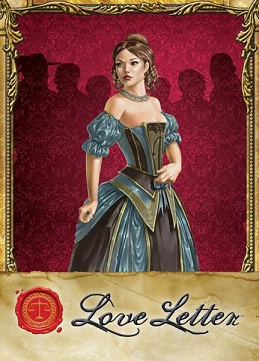
\includegraphics{Resources/ll_main_image.png}
	\caption{Love Letter - okładka} 
	\label{fig:llMainImage}
\end{figure}

\section{Opis zasad gry}
\label{sec:opisGry}
W trakcie gry wcielamy się w rolę jednego z adoratorów księżniczki starającego się o zdobycie jej serca. W tym celu przygotowaliśmy list miłosny, który chcemy jej dostarczyć. Niestety, księżniczka pogrążona jest obecnie w żałobie i nie przyjmuje do siebie nikogo obcego, w związku z czym musimy znaleźć inny sposób na przekazanie jej naszego listu. Oprócz księżniczki, na dworze znajdują się inne postacie, z których każda ma mniejszy lub większy dostęp do komnat naszej wybranki i może oddać jej list. Przekazujemy więc naszą przesyłkę swojemu tajnemu posłańcowi, a na koniec gry księżniczka jako pierwszy przeczyta ten list, który został przekazany przez najbardziej zaufaną postać. Serce wybranki zdobywa gracz, który jako pierwszy przekaże w ten sposób od 4 do 7 listów, w zależności od liczby graczy.

\section*{Cel i ustawienie początkowe rundy}
\label{sec:celIUstawieniePoczatkowe}
Love Letter rozgrywa się jako serię rund. Grę wygrywa gracz o następującej ilości wygranych rund:
\begin{itemize}
	\item 7 w grze na 2 graczy,
	\item 5 w grze na 3 graczy,
	\item 4 w grze na 4 graczy.
\end{itemize}
Każda runda dzieli się na tury, w których naprzemiennie jeden z graczy wykonuje ruch. Grę wygrywa ten z nich, który na końcu ostatniej tury posiada kartę o wyższym numerze.

Ustawienie początkowe każdej rundy wygląda następująco:
\begin{itemize}
	\item przetasuj karty
	\item odrzuć 1 wierzchnią kartę nie odkrywając jej (nie bierze udziału w rundzie),
	\item jeśli gra tylko 2 graczy, odrzuć 3 wierzchnie karty, odkryte,
	\item rozdaj po 1 karcie wszystkim graczom,
	\item jeśli jest to pierwsza runda, turę zaczyna gracz, który jako ostatni był na randce, w przeciwnym wypadku zaczyna zwycięzca poprzedniej rundy.
\end{itemize}

\section*{Tura gracza i opis kart}
\label{sec:turaGracza}
Podczas swojej tury gracz dociąga jedną kartę ze stosu. Następnie wybiera jedną z dwóch kart, które posiada już w ręce, kładzie ją przed sobą tak, by była widoczna dla wszystkich i zastosowuje opisany na niej efekt - nawet jeśli jest negatywny. Zagrana karta pozostaje odkryta przez całą rundę, a druga pozostaje w ręce. Następnie tura przechodzi na osobę po lewej stronie aktywnego gracza.

W grze znajduje się 16 kart, w 8 typach. Każda z typów kart posiada wartość od 1 do 8. Są to kolejno: 4 karty Strażniczki, po 2 karty Kapłana, Barona, Pokojówki i Księcia, oraz po jednej karcie Króla, Hrabiny i Księżniczki. Ich szczegółowy opis wraz z wyglądem znajduje się poniżej:

\clearpage
\begin{figure}[h]
	\centering
	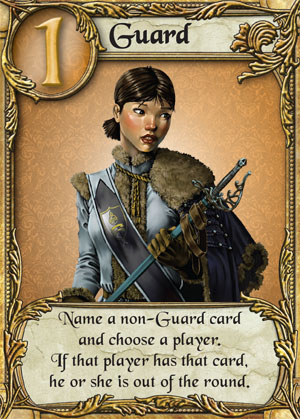
\includegraphics[scale=0.5]{Resources/Love_Letter_Card_Guard.png}
	\caption{Strażniczka} \label{fig:Love_Letter_Card_Guard}
\end{figure}
Na rysunku \ref{fig:Love_Letter_Card_Guard} przedstawiona jest karta typu Strażniczka. Zagrywając tę kartę należy wskazać jednego z pozostałych graczy i odgadnąć kartę którą posiada. Jeśli karta została prawidłowo odgadnięta, wskazany gracz odrzuca ją i przegrywa rundę.

\begin{figure}[h]
	\centering
	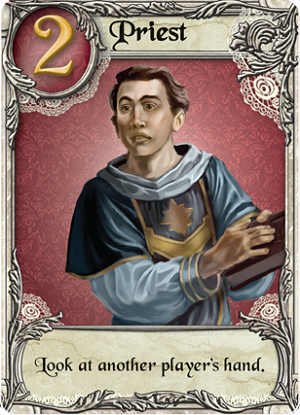
\includegraphics[scale=0.5]{Resources/Love_Letter_Card_Priest.png}
	\caption{Kapłan} \label{fig:Love_Letter_Card_Priest}
\end{figure}
Rysunek \ref{fig:Love_Letter_Card_Priest} przedstawia kartę typu Kapłan. Zagrywając tę kartę należy podglądnąć kartę wybranego gracza.

\clearpage
\begin{figure}[h]
	\centering
	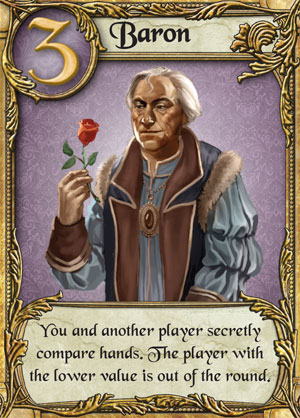
\includegraphics[scale=0.5]{Resources/Love_Letter_Card_Baron.png}
	\caption{Baron} \label{fig:Love_Letter_Card_Baron}
\end{figure}
Na rysunku \ref{fig:Love_Letter_Card_Baron} przedstawiona jest karta typu Baron. Po zagraniu tej karty należy w ukryciu porównać drugą posiadaną kartą z wybranym graczem. Następnie ten gracz, który ma kartę o mniejszej wartości odrzuca swoją kartę i przegrywa rundę. W przypadku remisu nic się nie dzieje.

\begin{figure}[h]
	\centering
	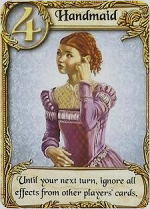
\includegraphics{Resources/Love_Letter_Card_Handmaid.png}
	\caption{Pokojówka} \label{fig:Love_Letter_Card_Handmaid}
\end{figure}
Rysunek \ref{fig:Love_Letter_Card_Handmaid} przedstawia kartę typu Pokojówka. Zagranie tej karty sprawia, że gracz jest niewrażliwy na efekt pozostałych kart do czasu swojej następnej tury.

\clearpage
\begin{figure}[h]
	\centering
	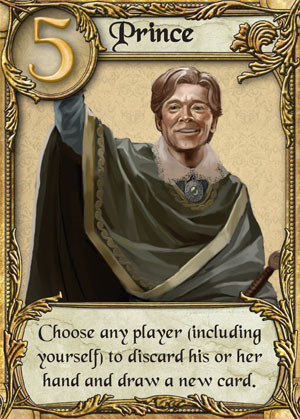
\includegraphics[scale=0.5]{Resources/Love_Letter_Card_Prince.png}
	\caption{Książe} \label{fig:Love_Letter_Card_Prince}
\end{figure}
Na rysunku \ref{fig:Love_Letter_Card_Prince} przedstawiona jest karta typu Książę. Zagranie pozwala wybrać dowolnego gracza (w tym siebie), zmusić go do odrzucenia posiadanej karty i pociągnięcia następnej.

\begin{figure}[h]
	\centering
	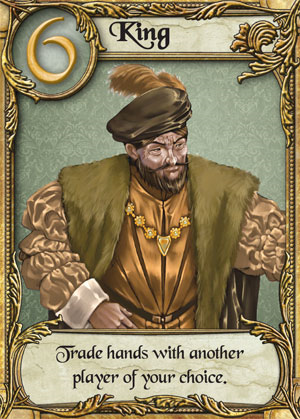
\includegraphics[scale=0.5]{Resources/Love_Letter_Card_King.png}
	\caption{Król} \label{fig:Love_Letter_Card_King}
\end{figure}
Rysunek \ref{fig:Love_Letter_Card_King} przedstawia kartę typu Król. Po jej zagraniu należy wymienić się drugą kartą z innym graczem.

\clearpage
\begin{figure}[h]
	\centering
	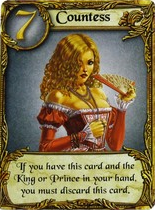
\includegraphics{Resources/Love_Letter_Card_Countess.png}
	\caption{Hrabina} \label{fig:Love_Letter_Card_Countess}
\end{figure}
Rysunek \ref{fig:Love_Letter_Card_Countess} przedstawia kartę typu Hrabina. Ta karta ma działanie pasywne. Nie wywiera efektu po zagraniu, natomiast zmusza gracza do jej zagrania jeśli równocześnie posiada na ręce kartę typu Książę lub Król.

\begin{figure}[h]
	\centering
	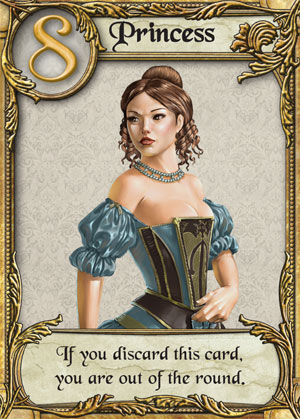
\includegraphics[scale=0.5]{Resources/Love_Letter_Card_Princess.png}
	\caption{Księżniczka} \label{fig:Love_Letter_Card_Princess}
\end{figure}
Na rysunku \ref{fig:Love_Letter_Card_Princess} przedstawiona jest karta typu Księżniczka. Zagranie tej karty oznacza natychmiastową przegraną w rundzie. Ta zasada działa również, gdy gracz został zmuszony do zagrania tej karty, np. przez efekt karty Książe.
\clearpage

\section{Definicja i analiza problemu}
\label{sec:opisProblemu}
Z wyżej przedstawionych zasad wynika, że gra cechuje się wysokim stopniem losowości i jest niedeterministyczna, więc można ją przedstawić jako problem optymalizacyjny$^{[\ref{bib:wiki_ProblemOptymalizacyjny}]}$. W związku z tym powstaje również pytanie, jaka jest najlepsza strategia mieszana$^{[\ref{bib:wiki_StrategiaTeoriaGier}]}$ maksymalizująca prawdopodobieństwo wygrania gry. Dla dalszych rozważań zakładam, że w gra toczy się pomiędzy dwoma graczami.

Najprostszym sposobem na znalezienie takiej strategii, byłoby stworzenie drzew probabilistycznych dla wszystkich możliwych stanów początkowych gry a następnie opracowanie algorytmu podejmowania decyzji opartego na danych statystycznych. Jednakże ilość i rozmiar tych drzew może być zbyt duża by znaleźć rozwiązanie problemu w rozsądnym czasie. Z tego powodu postanowiłem najpierw oszacować ile jest wszystkich możliwych przebiegów gry. Nim przejdę do obliczeń, wprowadzę kilka definicji by ustandaryzować używane pojęcia:
\begin{itemize}
	\item \textit{Decyzja} - inaczej \textit{Zagranie}, jest to typ karty wraz ze sposobem jej wykorzystania. Przykładowo: Zagranie karty typu Strażniczka z wyborem karty typu Król, lub zagranie karty typu Książę z wyborem na gracza przeciwnego.
	\item \textit{Podjęcie decyzji} - to wybór zagrania według zastosowanego algorytmu, które zostanie użyte jako ruch w grze.
	\item \textit{Strategia} - ciąg decyzji podejmowanych przez danych algorytm
	\item \textit{Scenariusz} - inaczej przebieg gry, chronologiczny ciąg decyzji podjętych przez obu graczy od początku do końca rundy; Jedna ze ścieżek w drzewie probabilistycznym dla danego stanu początkowego rundy.
\end{itemize}

\subsection*{Oszacowanie ilości rozwiązań}
Na przebieg każdej rundy wpływ mają następujące czynniki:
\begin{itemize}
	\item Kolejność kart w talii na początku rundy
	\item Zagrywanie kart przez graczy
\end{itemize}
Zacząłem od oszacowania ilości możliwych stanów początkowych. W każdej rundzie bierze udział wszystkie 16 kart. Zakładając, że każda z nich jest unikalna, to  liczba wszystkich możliwych kolejności kart to permutacja, którą obliczam wzorem podanym w [\ref{bib:tabliceMatematyczne}]:

\begin{center}
	$P_n = n!$ , gdzie $n\in N^+$
\end{center}

Dla  $n$ = 16, $n!=20 922 789 888 000$. Część kart się powtarza, więc tę liczbę należy jeszcze podzielić przez permutacje powtarzających się kart Strażniczki, Kapłana, Barona, Pokojówki oraz Księcia. Razem jest to $4! * 2! * 2! * 2! * 2! =  384$. Tak więc liczba unikalnych kolejności kart wynosi: 

\begin{center}
	$20 922 789 888 000 / 32 = 54486432000$ - 54mld, 864mln i 432 tys.
\end{center}

Nie jest to jednak ostateczne oszacowanie możliwych rozwiązań. W każdej turze gracz ma do wyboru co najmniej dwa zagrania, ponieważ tyle ma dostępnych kart. Jednakże, w przypadku karty Strażniczki możliwości jest więcej, ponieważ można wytypować 7 typów kart, a w jednym przypadku może to pokonać przeciwnika i skończyć rundę. W związku z tym, by oszacować liczbę rozwiązań przy ustalonym stanie początkowym, zastosowałem następujące ograniczenia:
\begin{itemize}
	\item zgodnie z zasadami gry dla dwóch graczy, odrzucam łącznie 4 pierwsze karty (1 zakryta, 3 odkryte).
	\item rozdaję po 1 karcie obu graczom. Pozostaje 10 kart w talii.
	\item zakładając, że żadna decyzja nie spowoduje zakończenia rundy, gracze łącznie 10 razy pociągną kartę, więc podejmą 10 decyzji.
	\item każdą decyzję można przedstawić jako 0 (zagranie posiadanej karty) lub 1 (zagranie pociągniętej karty) - w tym miejscu jeśli istnieje możliwość zagrania karty w wieloraki sposób, upraszczam to do jednego zagrania niekończącego rundę.
\end{itemize}
Na podstawie powyższego można oszacować, że możliwych rozwiązań dla danego stanu początkowego jest $2^{10}=1024$. Łącząc to z ilością stanów początkowych, utrzymujemy przybliżoną liczbę rozwiązań:

\begin{center}
	$54486432000 * 1024 = 55794106368000 \approx  5.6*10^{13}$
\end{center}

Z uwagi na rząd wielkości, stworzenie optymalnej strategii na podstawie analizy statystycznej wszystkich dostępnych rozwiązań byłoby czasochłonne. Z tego powodu, zamiast odpowiadać na pytanie ,,Jaka jest najlepsza strategia podejmowania decyzji?'', dużo łatwiej będzie odpowiedzieć na pytanie ,,która z podanych strategii jest najlepsza?''. Kierując się tą zasadą, w następnym rozdziale opisałem wybrane strategie, których skuteczność sprawdzę implementując je w napisanej przeze mnie aplikacji. Pozostaje jeszcze sformalizować przedstawiony problem za pomocą modelu matematycznego.


\section{Model matematyczny problemu}
W celu ujednolicenia używanych pojęć i skrótów, przedstawię je następująco:

\clearpage
\begin{table}[t]
	\caption{Pojęcia i skróty}
	\centering
	\begin{tabular}{|l|c|p{4cm}|c|}
		\hline
		\bf{Nazwa karty} & \bf{Skrót nazwy}  & \bf{Możliwe zagrania} & \bf{Skrót zagrania} \\ \hline
		Strażniczka & Str & Strażniczka z wyborem na [Nazwa karty] & Str\_Kap, Str\_Bar, ... , Str\_K-a  \\ \hline
		Kaplan & Kap & Zagranie kapłana & Kap\_Z \\ \hline
		Baron & Bar & Zagranie barona & Bar\_Z  \\ \hline
		Pokojówka & Pok & Zagranie pokojówki & Pok\_Z \\ \hline
		Książe & K-e & Książe na siebie; Książe na przeciwnika & K-e\_S, K-e\_P  \\ \hline
		Król & Krl & Zagranie Króla & Krl\_Z \\ \hline
		Hrabina & Hra & Hrabina, gdy druga karta w ręce to Król lub Książe; Zagranie Hrabiny & Hra\_K-e\_Kr, Hra\_Z \\ \hline
		Księżniczka & K-a & Zagranie Księżniczki & K-a\_Z \\ \hline
	\end{tabular}
\end{table}

Patrząc z perspektywy jednego z graczy, cała gra składa się z szeregu etapów(tur), gdzie w każdym etapie gracz podejmuje decyzje, a stan początkowy następnego etapu jest wynikiem dwóch akcji: podjętej decyzji (której efekt możemy przewidzieć z pewnym prawdopodobieństwem) i reakcji gracza drugiego, której prawdopodobieństwo jest nieokreślone. Dodatkowo, rzeczywisty stan każdego etapu nie jest w pełni znany graczowi. Z tych cech wynika, że grę ,,Love Letter'' możemy sklasyfikować jako \textbf{dynamiczny(wieloetapowy) proces podejmowania decyzji w warunkach niepewności}$^{[\ref{bib:matematyczneModeleKonfliktu_klasyfikacja}]}$. Jej zapis formalny można przedstawić jako grę w postaci ekstensywnej$^{[\ref{bib:matematyczneModeleKonfliktu_graEkstensywna}]}$:
\begin{center}
	$T = (S,R)$, gdzie
	\begin{itemize}
		\item $T$ - graf skierowany
		\item $S$ - zbiór wierzchołków (węzłów)
		\item $R$ - relacja określona na parach wierzchołków (łuki)
	\end{itemize}
\end{center}

Przypisując każdemu wierzchołkowi $s \in S$ jeden ze stanów rundy, a każdemu łukowi $r \in R$ ruch danego gracza lub udział losu, otrzymamy zapis pozwalający jednoznacznie określić możliwe przebiegi konkretnej gry, podjęte przez graczy decyzje, ich stan wiedzy na każdym etapie oraz wypłaty graczy (wynik gry).

Ponieważ w każdej rundzie bierze udział dwóch graczy, oznaczmy ich jako $P_1$ i $P_2$. Dodatkowo, część w której losowana jest karta oznaczmy jako $Los$. Zauważmy, że skoro korzeń $s_0$ to stan początkowy rundy przed losowaniem kart z talii, to wszystkie łuki wychodzące z $s_0$ są efektem losowania, a łuki z następnych poziomów należą kolejno do gracza $P_1$, $Losu$, gracza $P_2$ itd. Poglądowo zilustrowałem to w następujący sposób:

\clearpage
\begin{figure}[h]
	\centering
	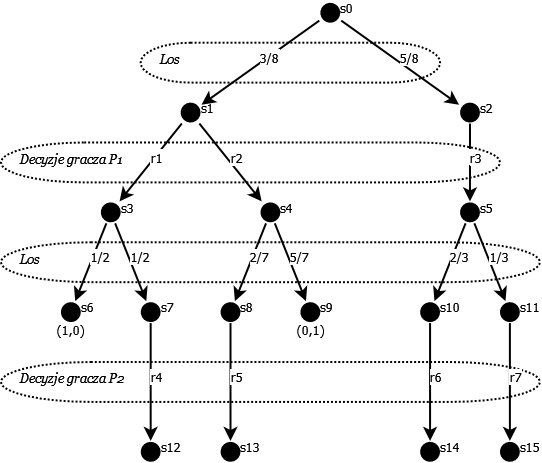
\includegraphics[scale=0.5]{Resources/drzewo.png}
	\caption{Pogląd gry w postaci ekstensywnej} \label{fig:drzewo}
\end{figure}
Ważne wnioski:
\begin{itemize}
	\item wszystkie łuki wychodzące z węzłów należących do $Losu$ oznaczone są prawdopodobieństwem sumującym się do 1.
	\item węzły $s_6$ i $s_9$ są liśćmi drzewa i zawierają wypłaty graczy (wynik gry) - 1 oznacza zwycięstwo, 0 oznacza przegraną. Przykładowo w węźle $s_6$ wygrał gracz $P_1$
	\item gracze nie wiedzą w jakim węźle danego poziomu się znajdują. Załóżmy, że łuki $r_4$ i $r_5$ są takim samym ruchem dostępnym dla gracza $P_2$. Ze względu na udział losu, gracz nie wie czy gra znajduje się w stanie $s_7$ czy $s_8$. Każda grupa takich stanów tworzy \textbf{zbiór informacyjny}. W dalszej części pracy takie zbiory będziemy określać jako $Inf$.
\end{itemize}

Przedstawiony model jednoznacznie określa stan gry i graczy. Dla uwzględnienia decyzyjności, do takiego modelu należy dodać jeszcze funkcję wyboru (decyzji). Oznaczmy ją jako $d$:
\begin{center}
	$d(Inf) = r$, gdzie $r$ jest dowolnym łukiem wychodzącym z
\end{center}
\clearpage
\begin{figure}[h]  % TODO poprawić by xn było xi na obrazku, bo i to |X|
	\centering
	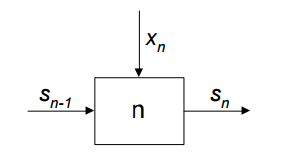
\includegraphics[]{Resources/Schemat_Modelu.png}
	\caption{Schemat modelu} \label{fig:Schemat_Modelu}
\end{figure}
\begin{itemize}
	\item n - etap gry
	\item $s_{n-1} \in S_{n-1}$ - stan wejściowy
	\item $x_i \in X_n$ - podjęta decyzja
	\item $s_{n} \in S_n$ - stan wyjściowy
	\item $X_n$ - zbiór dopuszczalnych decyzji dla etapu n-tego
	\item $S_n$ - zbiór dopuszczalnych stanów dla etapu n-tego
	\item $T_n: \{x_i, s_{n-1} \} \rightarrow \{s_n, X_n\}$ - funkcja przejścia
	\item $Q = max(P_w)$ - funkcja celu, gdzie $P_w$ oznacza prawdopodobieństwo wygranej
	\item $D: \{X_n, s_{n-1}\} \rightarrow x_n$ - strategia podejmowania decyzji
\end{itemize}
Funkcja przejścia $T_n$ wynika bezpośrednio z opisanych wcześniej zasad oraz zawiera reakcję gracza przeciwnego, w efekcie zwracając jeden z możliwych stanów należących do $S_n$ oraz zbiór dopuszczalnych decyzji $X_n$. Również wszystkie $S_0 .. S_n$ oraz $X_0 .. X_n$ wynikają z zasad gry. Jedynym nieokreślonym elementem pozostaje $D$, a moje propozycje na jego zdefiniowanie przedstawiam w następnym rozdziale.
\chapter{Przegląd wybranych algorytmów i innych rozwiązań}
\label{cha:rozdz3}

W tym rozdziale przedstawiam kilka wybranych algorytmów, które zaimplementuję w następnym rozdziale. Dla każdego z nich opisuję jego użycie w odniesieniu do gry 'Love Letter'.

\section{Algorytm losowy}
\label{sec:algLos}
\subsection{Opis}
Jest to najprostszy algorytm podejmowania decyzji. Na wejściu otrzymuje listę dostępnych zagrań, z których w całkowicie losowy sposób wybiera jedno. Każde z dostępnych zagrań ma takie samo prawdopodobieństwo bycia wybranym przez ten algorytm.

\subsection{Sposób wykorzystania}
Z uwagi na prostotę tego algorytmu, używam go jako punktu odniesienia dla wszystkich pozostałych strategii. Dla każdej z nich algorytm losowy spełnia rolę drugiego gracza i w ten sposób można łatwo porównać je ze sobą. Dla tego algorytmu zastosowałem jedną drobną modyfikację: nigdy nie podejmie decyzji o zagraniu Księżniczki - oznacza to natychmiastową przegraną niezależnie od momentu gry, co mogłoby mocno wypaczyć wyniki innych algorytmów.

\subsection{Zapis pseudokodem}
\begin{algorithmic}[1]
	\Function{$D_{losowa}$}{$X_n,s_{n-1}$}	
		\ForAll{ $x_i$ } 
			\If {$x_i ==$ Księżniczka}
				\State $X_n \gets X_n - x_i$
			\EndIf
		\EndFor
	\State \textbf{return} wylosujJeden($X_n$) 
	\EndFunction
\end{algorithmic}

\section{Algorytm zachłanny}
\label{sec:algZach}
\subsection{Opis}
Algorytm zachłanny polega na wyborze najlepszego możliwego zagrania dostępnego w danej chwili, nie analizując jego konsekwencji w przyszłości. Pomimo, że takie podejmowanie decyzji krótkowzroczne, jest łatwe w implementacji i daje atrakcyjne wyniki w niektórych problemach, np. przy szukaniu minimalnego drzewa rozpinającego\textsuperscript{[\ref{bib:algorytmy_zachlanny}]}.

\subsection{Sposób wykorzystania}

W kontekście gry 'Love Letter', implementacja algorytmu zachłannego wymaga pewnego doprecyzowania. Najważniejszą częścią jest funkcja kryterialna oceniająca wartość zagrania, która w niektórych przypadkach musi być oparta o probabilistykę wystąpienia kart u przeciwnika. 

Rozważmy przypadek, w którym algorytm musi podjąć decyzję o zagraniu karty Strażniczki, lub karty Barona. Jest to pierwszy ruch gracza, a w widocznych kartach odrzuconych na starcie są odrzucone karty Króla, Księcia i Pokojówki. Oznacza to, że w talii pozostało 9 kart, a jedna z odrzuconych jest niewidoczna, niemniej jednak ją też trzeba brać pod uwagę. Wyliczenie prawdopodobieństwa \textit{P} jaką kartę ma przeciwnik jest tym momencie proste, jednak trzeba jeszcze wziąć pod uwagę drobny szczegół - czy do liczenia \textit{P} wliczać karty posiadane w ręce. Z jednej strony wydaje się to nielogiczne i może prowadzić do wybierania nieoptymalnych decyzji (co przeczyłoby idei algorytmu zachłannego), z drugiej strony można to potraktować jako element blefu, który jest nieodłączną częścią każdej gry towarzyskiej. W swojej implementacji założyłem absolutną zachłanność algorytmu i karty posiadane na ręce są pomijane w obliczeniach. 
Wobec powyższego, prawdopodobieństwo wystąpienia kart u przeciwnika rozkłada się następująco:

\begin{table}[h]
	\caption{Przykład rozkładu prawdopodobieństwa}
	\centering
		\begin{tabular}{|l|r|}
			\hline
			\bf{Karta} & $P(Karta)$	\\ \hline
			Strażniczka & 30\% 			\\ \hline
			Kapłan & 20\% 				\\ \hline
			Baron & 10\% 				\\ \hline
			Pokojówka & 10\% 			\\ \hline
			Książę & 10\% 				\\ \hline
			Hrabina & 10\% 				\\ \hline
			Księżniczka & 10\% 			\\ \hline
		\end{tabular}
\end{table}

Zagranie karty Baron oznacza porównanie drugiej karty z kartą przeciwnika. Łatwo policzyć, że w 70\% przypadków skończyłoby to się porażką, a w 30\% nie było by żadnego efektu. Drugim dostępnym ruchem jest zagranie karty Strażniczki, a w jej przypadku najlepszym wyborem jest wytypowanie Kapłana, co daje 20\% szans na zwycięstwo i 80\% szans, że nie nastąpi żaden efekt. Zauważmy, że gdybyśmy wliczali posiadane karty do obliczenia prawdopodobieństwa, wystąpienie Barona i Kapłana byłoby tak samo możliwe. W takich przypadkach algorytm powinien zawsze celować w kartę z wyższym numerem. By formalnie stwierdzić, jaka decyzja powinna zostać podjęta, musimy obliczyć funkcję kryterialną dla dostępnych zagrań i wybrać to zagranie, dla której funkcja przyjmuje wyższy wynik. Przyjmijmy, że funkcja kryterialna wygląda następująco:

\begin{center}
	$F(Karta) = 1 + prawdopodobienstwo\_wygranej - prawdopodobienstwo\_przegranej$
\end{center}
Po podstawieniu otrzymujemy:
\begin{center}
 $F(Strazniczka)=1.2$ i $F(Baron) = 0.3$
 
 $F(Strazniczka)>F(Baron) => Decyzja=Zagranie(Pokojowka + Kaplan)$ 
\end{center} 

Najlepszą decyzją w tym wypadku jest zagranie karty Strażniczki z wyborem karty Kapłana. Jak jednak na podstawie powyższego wzoru ocenić zagranie karty Kapłana, Pokojówki lub Króla? Każda z nich wymaga unikalnej funkcji kryterialnej. Mając na uwadze, że w kontekście strategii zachłannej decyzja zawsze powinna być optymalna w ujęciu chwili, ustaliłem następujące warunki oceny zagrania karty:
\begin{itemize}
	\item Strażniczka - ocena zagrania wzrasta gdy pozwala wyeliminować przeciwnika.
	\item Kapłan - w ujęciu chwili jest to karta neutralna i ocena jej zagrania będzie zawsze stała.
	\item Baron - ocena zagrania wzrasta gdy mamy drugą kartę silniejszą niż może mieć przeciwnik.
	\item Pokojówka - podobnie jak w przypadku kapłana, ocena zagrania karty będzie stała.
	\item Książę - ocena zagrania na przeciwnika wzrasta z prawdopodobieństwem Księżniczki u przeciwnika. Ocena zagrania na siebie jest stała, lecz 0 gdy druga karta to Księżniczka.
	\item Król - ocena stała
	\item Hrabina - ocena stała, jednak musimy ją zagrać gdy druga posiadana karta to Król lub Książe
	\item Księżniczka - nie może być nigdy wyrzucona.
	\item Dodatkowo, jeśli oba zagrania mają taką samą wartość, powinna być podjęta decyzja o zagraniu karty o niższej wartości.
\end{itemize}

\subsection{Zapis pseudokodem}
\begin{algorithmic}[1]
	\Function{$D_{zachlanna}$}{$X_n,s_{n-1}$}
		\ForAll{ $rodzajKarty \in rodzajeKart$ } \Comment Tworzenie tablicy prawdopodobieństwa
			\State $P[rodzajKarty] \gets$  prawdopodobieństwo wystąpienia karty danego rodzaju u przeciwnika	
		\EndFor
		\State $ decyzja \gets NULL$ \Comment Szukanie zagrania o najwyższej wycenie
		\ForAll{ $x_i \in X_n$ } \Comment Obliczenie funkcji kryterialnej dla każdego zagrania
				\If {$F(decyzja, P[] < F(x_i, P[]$}
					\State $decyzja \gets x_i$
				\EndIf
		\EndFor		
		\State \textbf{return} $decyzja$
	\EndFunction
\end{algorithmic}

Gdzie funkcja kryterialna wygląda następująco:
\begin{algorithmic}[1]
	\Function{$F$}{$x_i,P[]$}	
		\Switch{$x_i$}
			\Case{Strażniczka + Kaplan} \Comment Zagranie Strażniczki na dany typ karty
				\State \textbf{return} $ 1 + P[Kaplan] + 0.08 $
			\EndCase
			\Case{Strażniczka + Baron}
				\State \textbf{return} $ 1 + P[Baron]  + 0.08 $
			\EndCase
			\State ...
			\Case{Strażniczka + Księżniczka}
				\State \textbf{return} $ 1 + P[Ksiezniczka]  + 0.08 $
			\EndCase
			\Case{Kapłan}
				\State \textbf{return} $ 1 + 0.07 $
			\EndCase
			\Case{Baron}	\Comment Kryterium zależy od wartości W() drugiej posiadanej karty (DK)
				\State $ szansePrzegranej \gets 0$ 
				\State $ szanseWygranej \gets 0$ 
				\ForAll {$typKarty$}
					\If {$ W(DK) < W(typKarty) $}  
						\State $szansePrzegranej \gets szansePrzegranej + P[typKarty]$ 
					\ElsIf {$ W(DK) > W(typKarty) $}
						\State $szanseWygranej \gets szanseWygranej + P[typKarty]$ 
					\EndIf
				\EndFor
				\State \textbf{return} $ 1 - szansePrzegranej + szanseWygranej + 0.06 $
			\EndCase
			\Case{Pokojówka}
				\State \textbf{return} $ 1 + 0.05 $
			\EndCase
			\Case{Książe na przeciwnika}
				\State \textbf{return} $ 1 + P[Ksiezniczka] + 0.04 $
			\EndCase
			\Case{Książe na siebie} 
				\If {$ DK == Ksiezniczka $}  
					\State \textbf{return} $ 0 $
				\Else
					\State \textbf{return} $ 1 + 0.04 $
				\EndIf
			\EndCase
			\Case{Król}
				\State \textbf{return} $ 1 + P[Ksiezniczka] + P[Hrabina] + 0.03 $
			\EndCase
			\Case{Hrabina, gdy druga posiadana karta to Król lub Książe}
				\State \textbf{return} $ 10 + 0.02 $
			\EndCase
			\Case{Hrabina}
				\State \textbf{return} $ 1 + 0.02 $
			\EndCase
			\Case{Księżniczka}
				\State \textbf{return} $ 0 $
			\EndCase
		\EndSwitch
	\EndFunction
\end{algorithmic}


\section{Algorytm min-max}
\label{sec:minmax}
\subsection{Opis}
Algorytm minimaksowy polega na ,,minimalizowaniu maksymalnych możliwych strat'' bądź alternatywnie na ,,maksymalizacji minimalnego zysku''$^{[\ref{bib:wiki_minMax}]}$. Zgodnie z [\ref{bib:wazniak_minMax}] często stosuje się go do gier o następujących zasadach:
\begin{itemize}
	\item występuje dwóch graczy
	\item ruchy wykonywane są naprzemiennie
	\item w każdym stanie istnieje skończona liczba decyzji do podjęcia
	\item stan i podjęta decyzja jednoznacznie wyznaczają stan następny
	\item każdy stan może zakwalifikować do jednej z następujących kategorii:
	\begin{itemize}
		\item wygrana pierwszego gracza
		\item wygrana drugiego gracza
		\item remis
		\item sytuacja nierozstrzygnięta
	\end{itemize}
\end{itemize}

\subsection{Sposób wykorzystania}
W podanym powyżej opisie, gra Love Letter niezgodna jest w punkcie czwartym. Ze względu na niepewność jaką kartę posiada przeciwnik, jaką pociągnie ze stosu w swojej turze, oraz jaki wykona ruch, podjęcie decyzji $x_i$ w stanie $s_{n-1}$ nie określa jednoznacznie stanu $s_n$. Mimo to, jesteśmy w stanie statystycznie ocenić możliwości przeciwnika, a tym samym zminimalizować naszą maksymalną stratę. Ponieważ zysk należy rozumieć jako zwiększenie szansy na wygraną (tak jak w strategii zachłannej), to strata oznacza zwiększenie szansy na przegraną. 

Rozważmy scenariusz, w którym gracz pierwszy posiada kartę Księcia oraz Pokojówki. Na stosie pozostało 2 karty, 1 karta jest zakryta zgodnie z zasadami rozpoczęcia rundy i przeciwnik również posiada 1 kartę. Wśród tych 4 nieznanych graczowi kart są karty Strażniczki, Barona, Księcia oraz Księżniczki. Prawdopodobieństwo wystąpienia każdej z nich u przeciwnika wynosi 25\% i razem stanowią one tablicę prawdopodobieństwa $P[]$. Przyjmijmy, że wykorzystywana w poprzedniej strategii funkcja kryterialna $F(Karta, P[])$ to maksymalizacja zysku i nazwijmy ją $F_{max}(Karta, P[])$  Zgodnie z jej definicją $F_{max}(Ksiaze, P[]) = 1.29$ i $F_{max}(Pokojowka, P[]) = 1.05$, więc zagranie Księcia maksymalizuje szansę na wygraną. Jeśli jednak weźmiemy pod uwagę, że w 75\% przypadków nie wygrywamy, wówczas musimy rozważyć odpowiedź przeciwnika. W tym wypadku jest 6 par kart które może posiadać przeciwnik, więc dla każdej z nich, zgodnie ze strategią zachłanną, należy obliczyć funkcję kryterialną oraz szansę na przegraną. Dodatkowo należy zauważyć, że z perspektywy przeciwnika w każdym przypadku gracz pierwszy ma inny rozkład prawdopodobieństwa wystąpienia karty. Pełne obliczenia znajdują się w tabeli poniżej.
\begin{center}
	Skróty : \textit{Str} - Strażniczka; \textit{Bar} - Baron; \textit{Pok}-Pokojówka; \textit{K-e} - Książę; \textit{K-a} - Księżniczka
	
	
	Gracz pierwszy po zagraniu Księcia posiada kartę Pokojówki.
\end{center}
\begin{table}[h]
	\caption{Scenariusze reakcji przeciwnika na decyzję w stanie $s_{n-1}$}
	\centering
	\begin{tabular}{|l|c|r|r|r|}
		\hline
		\bf{Karty 1 i 2} & $P(Karta)$ pierwszego gracza  & $F(Karta_1)$ & $F(Karta_2)$ & Szanse przegranej	\\ \hline
		Str ; Bar & $P(\textit{Pok}) = P(\textit{K-e}) = P(\textit{K-a}) = 33.(3)\%$ & 1.41 & 0.6	& 33.(3)\% \\ \hline
		Str ; K-e & $P(\textit{Pok}) = P(\textit{Bar}) = P(\textit{K-a}) = 33.(3)\%$ & 1.41 & 1.37 & 33.(3)\%	\\ \hline
		Str ; K-a & $P(\textit{Str}) = P(\textit{Bar}) = P(\textit{K-e}) = 33.(3)\%$ & 1.41 & 0 & 33.(3)\% \\ \hline
		Bar ; K-e & $P(\textit{Str}) = P(\textit{Pok}) = P(\textit{K-a}) = 33.(3)\%$ & 1.39 & 1.37 & 100\% \\ \hline
		Bar ; K-a & $P(\textit{Str}) = P(\textit{Pok}) = P(\textit{K-e}) = 33.(3)\%$ & 2.06 & 0 & 100\% \\ \hline
		K-e ; K-a & $P(\textit{Str}) = P(\textit{Pok}) = P(\textit{Bar}) = 33.(3)\%$ & 1.04 & 0 & 0\% \\ \hline
	\end{tabular}
\end{table}
Każdy rozważany scenariusz ma taką samą szansę wystąpienia, czyli $\frac{1}{6}$. Statystycznie szansa na przegraną wynosi więc:
\begin{center}
 $\frac{1}{6} * (\frac{1}{3} + \frac{1}{3} + \frac{1}{3} + 1 + 1 + 0) = \frac{1}{6} * 3 = 0.50 $
\end{center}
Warunkiem wystąpienia możliwości przegrania, jest brak wygranej po zagraniu Księcia, czyli ostatecznie szanse na przegraną wynoszą:
\begin{center}
	$F_{min}(Ksiaze, P[]) = 0.75 * 0.50 = 0.375$
\end{center}
Modyfikując o tę wartość ocenę zagrania Księcia otrzymujemy finalnie:
\begin{center}
	$K(Ksiaze) =  F_{max}(Ksiaze, P[]) - F_{min}(Ksiaze, s_{n-1}) = 1.29 - 0.375 = 0.915$
\end{center} 
W przypadku zagrania Pokojówki szanse przegrania wynoszą 0\%, ponieważ zgodnie z zasadami gry jesteśmy odporni na działanie kart przeciwnika:
\begin{center}
	$K(Pokojowka) =  F_{max}(Pokojowka, P[]) - F_{min}(Pokojowka, s_{n-1}) = 1.05 - 0 = 1.05$
\end{center} 
Wynika z tego, że decyzją która minimalizuje maksymalną stratę jest $Zagranie(Pokojowka)$.

\subsection{Zapis pseudokodem}
\begin{algorithmic}[1]
	\Function{$D_{minimaksowa}$}{$X_n,s_{n-1}$}
		\ForAll{ $rodzajKarty \in rodzajeKart$ } \Comment Tworzenie tablicy prawdopodobieństwa
			\State $P[rodzajKarty] \gets$  prawdopodobieństwo wystąpienia karty danego rodzaju u przeciwnika	
		\EndFor
		\ForAll{ $x_i \in X_n$ } \Comment Obliczenie funkcji kryterialnej dla każdego zagrania
			\State $K[x_i] \gets F_{max}(x_i, P[]) - F_{min}(x_i, s_{n-1})$
		\EndFor		
		\State $ decyzja \gets x_0$ \Comment Szukanie zagrania o najwyższej wycenie
		\ForAll{ $x_i$ } 
			\If {$K[decyzja] < K[x_i]$}
				\State $decyzja \gets x_i$
			\EndIf
		\EndFor		
		\State \textbf{return} $decyzja$
	\EndFunction
\end{algorithmic}

Funkcja $F_{max}(Karta)$ jest identyczna do $F(Karta)$ występującej w strategii zachłannej, w związku z czym zapiszę wyłącznie $F_{min}(Karta$).
\begin{algorithmic}[1]
	\Function{$F_{min}$}{$x_i, s_{n-1}$}	
		\State $L[Y_n] \gets$ lista możliwych zbiorów decyzji przeciwnika 
		\Switch{$x_i$}
			\Case{Strażniczka + Kaplan} \Comment Szanse, że Strażniczka nie przyniesie zwycięstwa
				\State \textbf{return} $ (1 - P[Kaplan]) * R(s_{n-1}, L[Y_n]) $
			\EndCase
			\Case{Strażniczka + Baron}
				\State \textbf{return} $ (1 - P[Baron]) * R(s_{n-1}, L[Y_n]) $
			\EndCase
				\State ...
			\Case{Strażniczka + Księżniczka}
				\State \textbf{return} $ (1 - P[Ksiezniczka]) * R(s_{n-1}, L[Y_n]) $
			\EndCase
			\Case{Kapłan}
				\State \textbf{return} $  R(s_{n-1}, L[Y_n]) $
			\EndCase
			\Case{Baron}	\Comment Szanse, że porównanie zakończy się remisem 
				\State $ szanseRemisu \gets P[DK]$ 
				\State \textbf{return} $ szanseRemisu * R(s_{n-1}, L[Y_n]) $
			\EndCase
			\Case{Pokojówka}
				\State \textbf{return} $ 0 $
			\EndCase
			\Case{Książe na przeciwnika}
				\State \textbf{return} $ (1 - P[Ksiezniczka]) * R(s_{n-1}, L[Y_n]) $
			\EndCase
			\Case{Książe na siebie} 
				\If {$ DK == Ksiezniczka $}  
					\State \textbf{return} $ 0 $
				\Else
					\State \textbf{return} $ R(s_{n-1}, L[Y_n]) $
				\EndIf
			\EndCase
			\Case{Król}
				\State \textbf{return} $ R(s_{n-1}, L[Y_n]) $
			\EndCase
			\Case{Hrabina, gdy druga posiadana karta to Król lub Książe}
				\State \textbf{return} $ R(s_{n-1}, L[Y_n]) $
			\EndCase
			\Case{Hrabina}
				\State \textbf{return} $ R(s_{n-1}, L[Y_n]) $
			\EndCase
				\Case{Księżniczka}
			\State \textbf{return} $ 0 $
			\EndCase
		\EndSwitch
	\EndFunction
\end{algorithmic}

Funkcja $R(s_{n-1}, L[Y_n])$ oznacza szansę porażki po reakcji przeciwnika.
\begin{algorithmic}[1]
	\Function{$R$}{$s_{n-1}, L[Y_n]$}
		\ForAll {$Y_n \in L[X_n]$}
			\State $Z[] \gets D_{zachlanna}(Y_n, s_{n-1}) $	\Comment Lista potencjalnych reakcji
		\EndFor
		\ForAll {$x_i \in Z[]$}	\Comment Sprawdzenie szansy porażki
			\Switch{$x_i$}
				\Case{Strazniczka + DK}	\Comment DK - druga karta pierwszego gracza
					\State $P_{porazki}[x_i] \gets (Z[x_i] - 1.08)$
				\EndCase
				\Case{Baron}
					\If{$W(DK) < W(DK_{przeciwnika})$}
						\State $P_{porazki}[x_i] \gets 1$
					\Else
						\State $P_{porazki}[x_i] \gets 0$
					\EndIf
				\EndCase
				\Case{Książę}
					\If{$DK == Ksiezniczka$}
						\State $P_{porazki}[x_i] \gets 1$
					\Else
						\State $P_{porazki}[x_i] \gets 0$
					\EndIf
				\EndCase
			\EndSwitch
		\EndFor
		\State \textbf{return} $ \sum_{i=0}^{Z[].size} \frac{1}{Z[].size} * P_{porazki}[i] $
	\EndFunction
\end{algorithmic}
\section{Algorytm Monte Carlo Tree Search}
\label{sec:algMCTS}
\chapter{Implementacja}
\label{cha:rozdz4}

\section{Analiza wymagań}
Implementacja zasad i modelu przedstawionego w w rozdziale 2. Use case'y - wybór dwóch S.I. które będą przeciwko sobie grać, ustalanie ilości partii, parametryzacja MCTS (przeciwnik, czas na ruch). Program ma zwracać statystyki zwycięstw.
\section{Koncepcja wykonania}
Java w konsoli. Albo Python. Się zobaczy.

\section{Wykorzystane technologie}
j. w.

\section{Diagramy}
Wrzucić use case'y, UML klas,

\section{Prezentacja systemu}
Parę screenów z wynikami.

\section{Problemy napotkane w trakcie realizacji}
Czas, czas, czas.
\chapter{Rezultaty}
\label{cha:rozdz5}

W tym rozdziale zamieszczam rezultaty eksperymentów symulacyjnych z użyciem opisanych wcześniej algorytmów. Dla każdego z nich przedstawiam średni procent zwycięstw oraz zagrania, które najczęściej kończyły grę. Początkowo prezentuję statystyki z eksperymentów w których każdy z algorytmów gra z algorytmem losowym, będącym zawsze jest drugim graczem. Następne prezentuję wyniki z eksperymentów, w których biorą udział algorytm zachłanny, algorytm minimaksowy i algorytm MCTS. W tych przypadkach eksperyment ustawiony jest tak, by każdy z algorytmów był naprzemiennie pierwszym i drugim graczem. Rozdział kończę opisaniem wniosków ogólnych oraz z działania poszczególnych algorytmów.
W każdym porównaniu prezentuję statystyki oparte na próbie 100 tysięcy  symulacji, z wyjątkiem tych, gdzie porównywany jest algorytm MCTS. Dla tych przypadków, ze względu na czas trwania jednej rozgrywki, ograniczyłem próbę do 1 tysiąca.

\section{Algorytm losowy versus Algorytm Losowy}

\begin{figure}[H]
	\centering
	\includegraphics[width=\textwidth]{Resources/RVsR/RVsRwin.PNG}
	\caption{Wykres kołowy zwycięstw i remisów} 
	\label{fig:RVsRwin}
\end{figure}

Powyższy wykres na rys. \ref{fig:RVsRwin} wskazuje na pewną przewagę gracza rozpoczynającego.

\begin{figure}[H]
	\centering
	\includegraphics[width=\textwidth]{Resources/RVsR/RVsRroundwin.PNG}
	\caption{Wykres wygranych w danej rundzie} 
	\label{fig:RVsRroundwin}
\end{figure}

Na rys. \ref{fig:RVsRroundwin} widać wyraźną tendencję do spadku zakończeń gry wraz z kolejnymi rundami, za wyjątkiem przedostatniej, gdzie następuje wzrost.

\clearpage
\begin{figure}[H]
	\centering
	\includegraphics[width=\textwidth]{Resources/RVsR/RVsRdecision.PNG}
	\caption{Wykres zwycięskich zagrań} 
	\label{fig:RVsRdecision}
\end{figure} 

\begin{figure}[H]
	\centering
	\includegraphics[width=\textwidth]{Resources/RVsR/RVsRguarddecision.PNG}
	\caption{Wykres szczegółowy zwycięskich zagrań karty Strażniczki} 
	\label{fig:RVsRguarddecision}
\end{figure}

Z dwóch powyższych wykresów (rys. \ref{fig:RVsRdecision} i rys. \ref{fig:RVsRguarddecision}) wynika, że zdecydowanie najczęstszym wygrywającym ruchem jest zagranie karty Baron. Około połowę mniej zwycięstw jest w wyniku zagrania karty Strażniczki. Warty uwagi jest fakt, że im bliżej końca gry tym częściej zwycięskim zagraniem jest zagranie karty Księcia na przeciwnika.

\section{Algorytm zachłanny versus Algorytm losowy}

\begin{figure}[H]
	\centering
	\includegraphics[width=\textwidth]{Resources/GVsR/GVsRwin.PNG}
	\caption{Wykres kołowy zwycięstw i remisów} 
	\label{fig:GVsRwin}
\end{figure}

Powyżej (rys. \ref{fig:GVsRwin}) widać zauważalną przewagę algorytmu zachłannego nad losowym.

\begin{figure}[H]
	\centering
	\includegraphics[width=\textwidth]{Resources/GVsR/GVsRroundwin.PNG}
	\caption{Wykres wygranych w danej rundzie} 
	\label{fig:GVsRroundwin}
\end{figure}

Na rys. \ref{fig:GVsRroundwin} widać różnicę w porównaniu do eksperymentu poprzedniego, gdzie obaj gracze grają losowo. Nie ma tak wyraźnego wzrostu liczby gier skończonych w przedostatniej rundzie. Wynika to ze znacznie mniejszej ilości gier zakończonych remisem.

\clearpage
\begin{figure}[H]
	\centering
	\includegraphics[width=\textwidth]{Resources/GVsR/GVsRdecision.PNG}
	\caption{Wykres zwycięskich zagrań} 
	\label{fig:GVsRdecision}
\end{figure} 

\begin{figure}[H]
	\centering
	\includegraphics[width=\textwidth]{Resources/GVsR/GVsRguarddecision.PNG}
	\caption{Wykres szczegółowy zwycięskich zagrań karty Strażniczki} 
	\label{fig:GVsRguarddecision}
\end{figure}
Wykres \ref{fig:GVsRdecision} pokazuje niewielkie zróżnicowanie zwycięskich zagrań, za wyjątkiem ostatniej tury. Wskazuje to na tendencję algorytmu zachłannego do wyeliminowania przeciwnika, kiedy tylko jest to możliwe.
Porównanie wykresów na rysunkach \ref{fig:RVsRguarddecision} oraz \ref{fig:GVsRguarddecision} pokazują ogromny wzrost znaczenia zagrania karty Strażniczki z wyborem karty Książę. Algorytm zachłanny osiąga zwycięstwo zagrywając Strażniczkę niemal tak samo często co przy zagraniu Barona.

\section{Algorytm minimaksowy versus Algorytm losowy}

\begin{figure}[H]
	\centering
	\includegraphics[width=\textwidth]{Resources/MmVsR/MmVsRwin.PNG}
	\caption{Wykres kołowy zwycięstw i remisów} 
	\label{fig:MmVsRwin}
\end{figure}

Powyższy wykres (rys. \ref{fig:MmVsRwin}) pokazuje dużą przewagę algorytmu minimaksowego nad algorytmem losowym.

\begin{figure}[H]
	\centering
	\includegraphics[width=\textwidth]{Resources/MmVsR/MmVsRroundwin.PNG}
	\caption{Wykres wygranych w danej rundzie} 
	\label{fig:MmVsRroundwin}
\end{figure}

Wykres na rys. \ref{fig:MmVsRroundwin} pokazuje wyraźną tendencję do spadku średniej liczby wygranych gier wraz z kolejnymi turami, co występuje również u algorytmu zachłannego.

\begin{figure}[H]
	\centering
	\includegraphics[width=\textwidth]{Resources/MmVsR/MmVsRdecision.PNG}
	\caption{Wykres zwycięskich zagrań} 
	\label{fig:MmVsRdecision}
\end{figure} 

Wykres na rysunku \ref{fig:MmVsRdecision} pokazuje, że najskuteczniejszym zagraniem jest zagranie karty Baron. 

\begin{figure}[H]
	\centering
	\includegraphics[width=\textwidth]{Resources/MmVsR/MmVsRguarddecision.PNG}
	\caption{Wykres szczegółowy zwycięskich zagrań karty Strażniczki} 
	\label{fig:MmVsRguarddecision}
\end{figure}

Na rys. \ref{fig:MmVsRguarddecision} widać, że zagranie karty Strażniczki daje najwięcej zwycięstw gdy jest zagrana z wyborem na kartę Księcia. Zdecydowanie mniej korzystny jest wybór karty Pokojówki i Barona.

\section{Algorytm MCTS versus Algorytm Losowy}
Dane z eksperymentów symulacyjnych, w których bierze udział algorytm MCTS, opierają się na próbie 1000 gier, ponieważ większa próba znacząco zwiększa czas oczekiwania na wyniki. Wynika to z charakteru algorytmu, który działa przez zadany czas. W przeprowadzonych symulacjach czas działania algorytmu ustawiony był na 100ms.

\begin{figure}[H]
	\centering
	\includegraphics[width=\textwidth]{Resources/MctsVsR/MctsVsRwin.PNG}
	\caption{Wykres kołowy zwycięstw i remisów} 
	\label{fig:MctsVsRwin}
\end{figure}

Powyższy wykres (rys. \ref{fig:MctsVsRwin}) pokazuje w tym wypadku zauważalną przewagę algorytmu losowego nad algorytmem Monte Carlo Tree Search, mimo, że był drugim graczem. Spowodowane jest to między innymi błędnie przyjętym założeniem, że podstawowa forma algorytmu MCTS osiągnie dobre wyniki mimo czynnika losowego, o ile ilość symulacji na turę będzie odpowiednio duża.

\begin{figure}[H]
	\centering
	\includegraphics[width=\textwidth]{Resources/MctsVsR/MctsVsRroundwin.PNG}
	\caption{Wykres wygranych w danej rundzie} 
	\label{fig:MctsVsRroundwin}
\end{figure}

Wykres na rys. \ref{fig:MctsVsRroundwin} pokazuje, że średnia liczba zwycięstw wzrasta w ostatnich turach, co jest charakterystyczne również dla eksperymentu z dwoma algorytmami losowymi.

\begin{figure}[H]
	\centering
	\includegraphics[width=\textwidth]{Resources/MctsVsR/MctsVsRdecision.PNG}
	\caption{Wykres zwycięskich zagrań} 
	\label{fig:MctsVsRdecision}
\end{figure} 

\begin{figure}[H]
	\centering
	\includegraphics[width=\textwidth]{Resources/MctsVsR/MctsVsRguarddecision.PNG}
	\caption{Wykres szczegółowy zwycięskich zagrań karty Strażniczki} 
	\label{fig:MctsVsRguarddecision}
\end{figure}

Wykresy na rysunkach \ref{fig:MctsVsRdecision} i \ref{fig:MctsVsRguarddecision} pokazują wyraźną tendecję algorytmu MCTS do zagrywania karty Strażniczki z wyborem na Kapłana.

\section{Algorytm Minimaksowy versus Algorytm Zachłanny}
\begin{figure}[H]
	\centering
	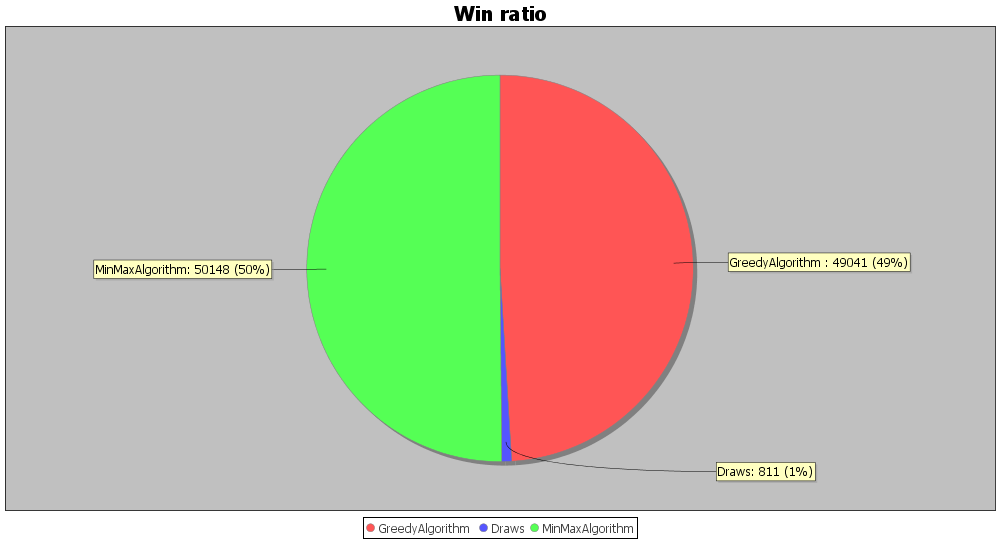
\includegraphics[width=\textwidth]{Resources/MirrorMmVsG/GVsMmWin.PNG}
	\caption{Wykres kołowy zwycięstw i remisów} 
	\label{fig:MirrorGVsMmWin}
\end{figure}

\begin{figure}[H]
	\centering
	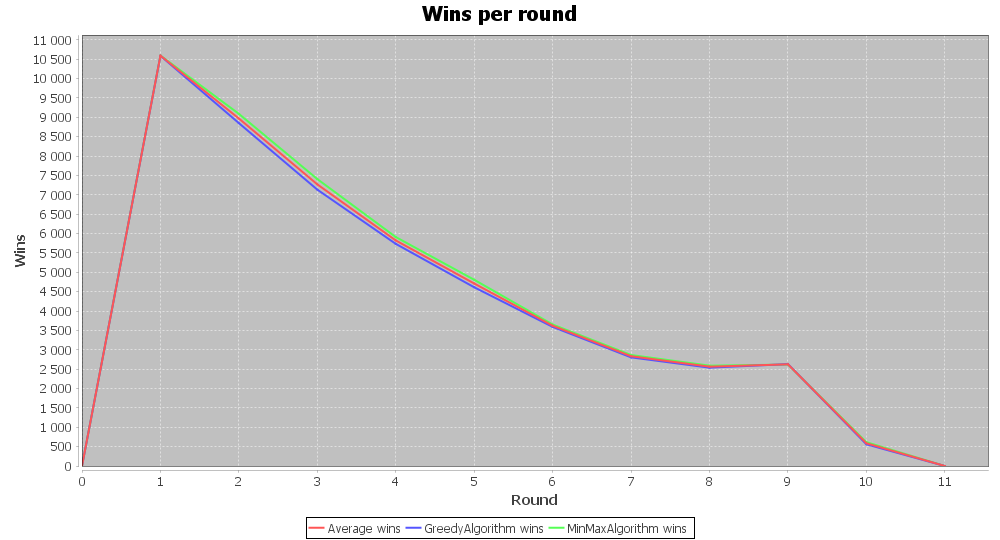
\includegraphics[width=\textwidth]{Resources/MirrorMmVsG/GVsMmRoundWin.PNG}
	\caption{Wykres wygranych w danej rundzie} 
	\label{fig:MirrorGVsMmRoundWin}
\end{figure}

Powyższe wykresy (rys. \ref{fig:MirrorGVsMmWin} i \ref{fig:MirrorGVsMmRoundWin}) pokazują niewielką przewagę algorytmu minimaksowego nad zachłannym, który przeważa w rundach od 1 do 8. W rundach 9 i 10 przeważa algorytm zachłanny, z czego wynika, że częściej wygrywa gry kończące się porównaniem siły kart.

\begin{figure}[H]
	\centering
	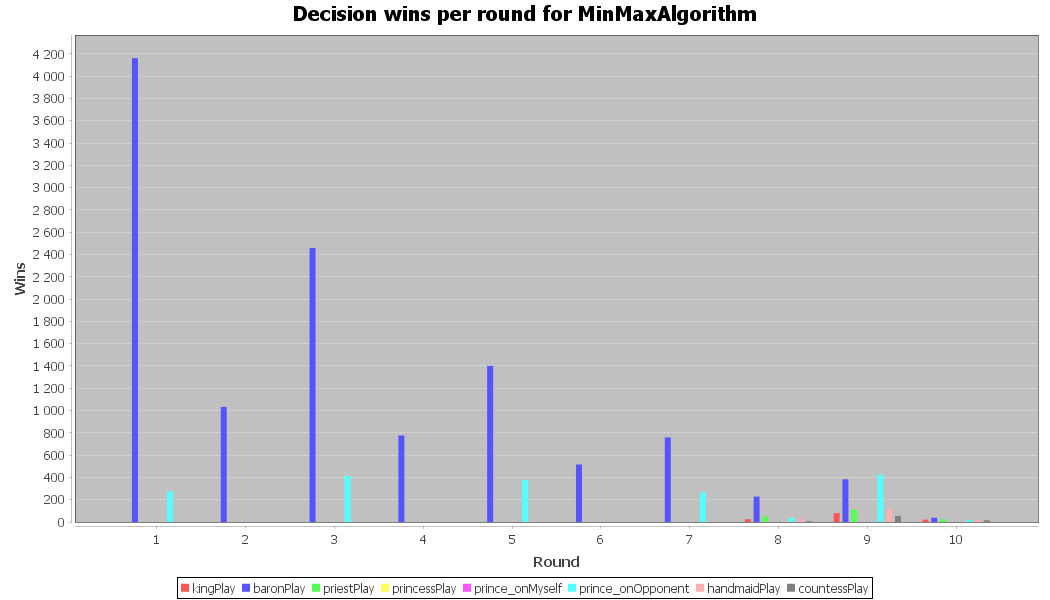
\includegraphics[width=\textwidth]{Resources/MirrorMmVsG/MmVsGDecision.PNG}
	\caption{Wykres zwycięskich zagrań} 
	\label{fig:MirrorMmVsGDecision}
\end{figure} 

\begin{figure}[H]
	\centering
	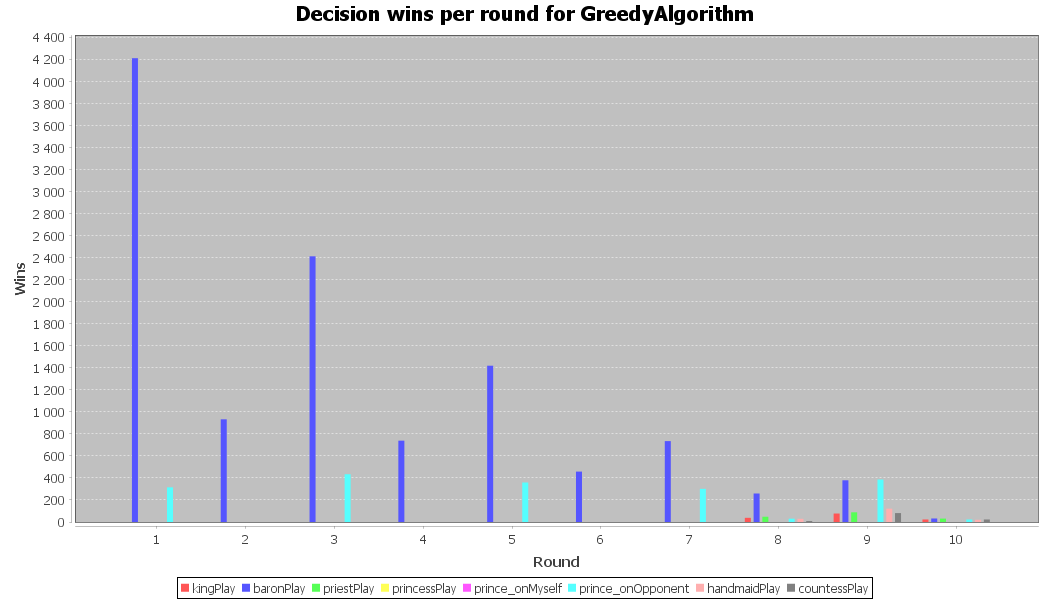
\includegraphics[width=\textwidth]{Resources/MirrorMmVsG/GVsMmDecision.PNG}
	\caption{Wykres zwycięskich zagrań} 
	\label{fig:MirrorGVsMmDecision}
\end{figure} 

\begin{figure}[H]
	\centering
	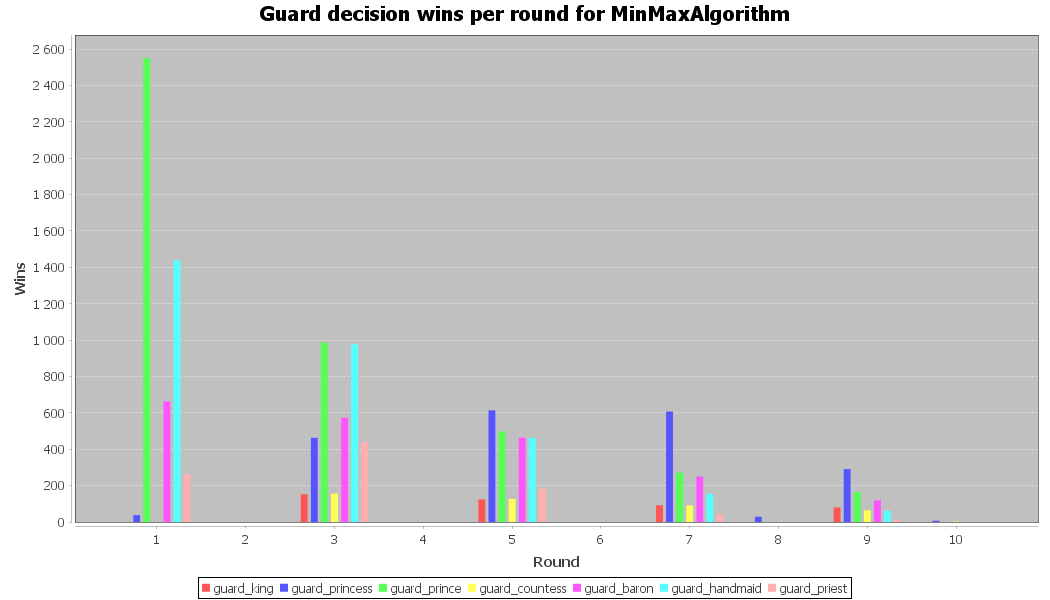
\includegraphics[width=\textwidth]{Resources/MirrorMmVsG/MmVsGGuardDecision.PNG}
	\caption{Wykres szczegółowy zwycięskich zagrań karty Strażniczki} 
	\label{fig:MmVsGGuardDecisionn}
\end{figure}

\begin{figure}[H]
	\centering
	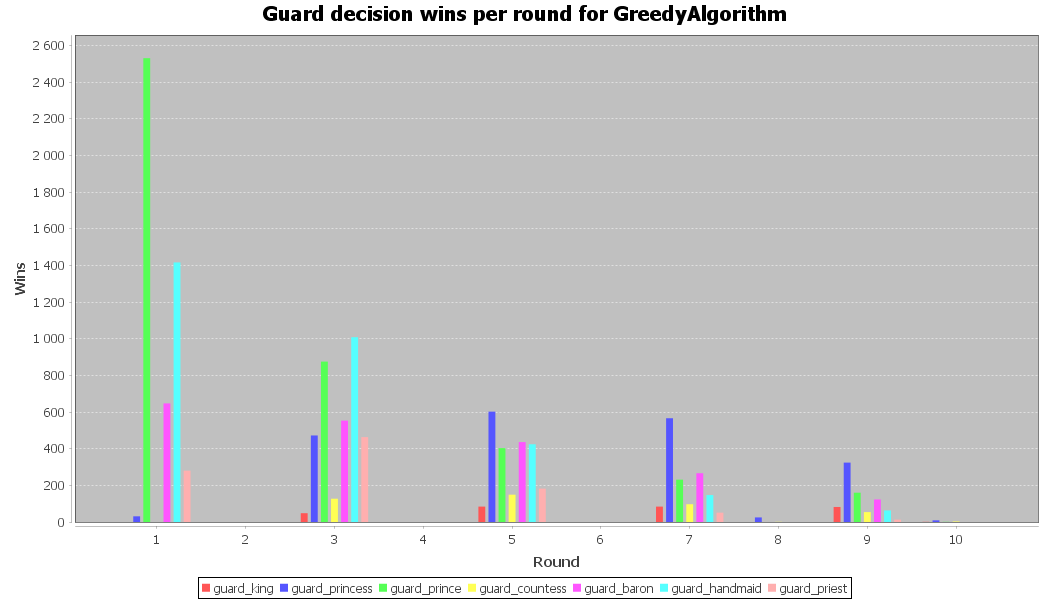
\includegraphics[width=\textwidth]{Resources/MirrorMmVsG/GVsMmGuardDecision.PNG}
	\caption{Wykres szczegółowy zwycięskich zagrań karty Strażniczki} 
	\label{fig:GVsMmGuardDecision}
\end{figure}


Z wykresów na rysunkach \ref{fig:MirrorMmVsGDecision}, \ref{fig:MirrorGVsMmDecision}, \ref{fig:MmVsGGuardDecisionn} i \ref{fig:GVsMmGuardDecision} wynika, że oba algorytmy wykazują duże podobieństwa - najczęściej wygrywają poprzez zagranie karty Barona, a zagrywając kartę Strażniczki najczęściej wybierają kartę Księcia.
\clearpage
\section{Algorytm Zachłanny versus Algorytm MCTS}

\begin{figure}[H]
	\centering
	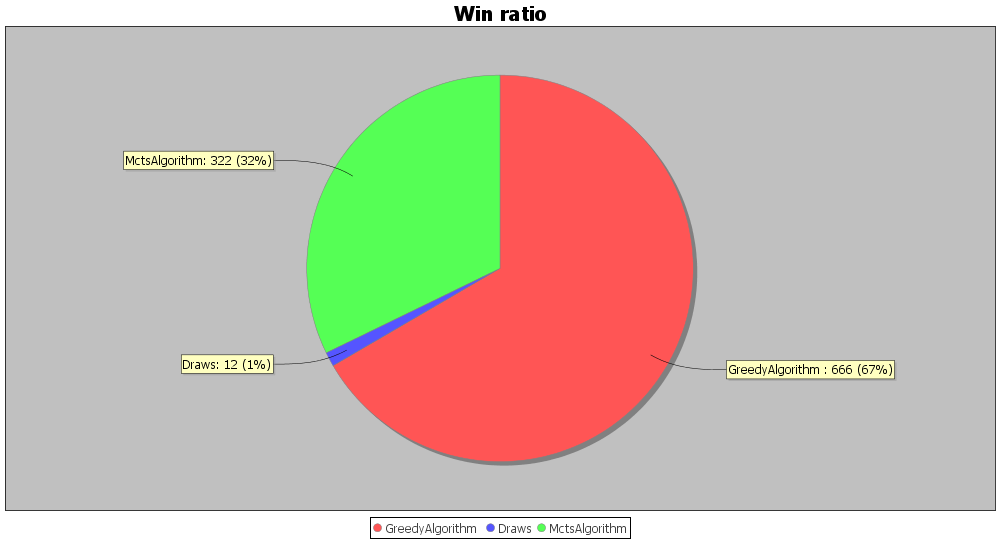
\includegraphics[width=\textwidth]{Resources/MirrorMctsVG/GVsMctsWin.PNG}
	\caption{Wykres kołowy zwycięstw i remisów} 
	\label{fig:GVsMctsWin}
\end{figure}

\begin{figure}[H]
	\centering
	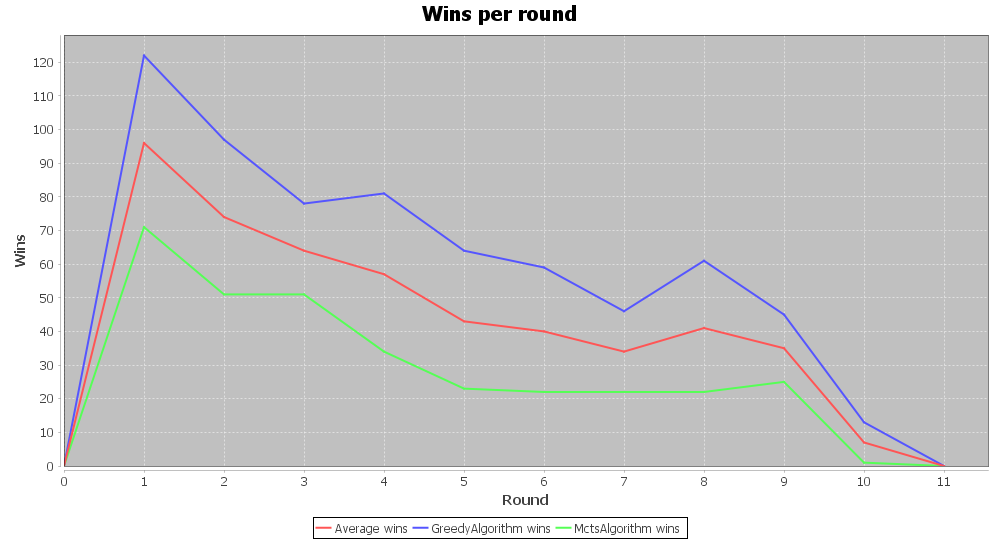
\includegraphics[width=\textwidth]{Resources/MirrorMctsVG/GVsMctsRoundWin.PNG}
	\caption{Wykres wygranych w danej rundzie} 
	\label{fig:GVsMctsRoundWin}
\end{figure}

Powyższe wykresy (rys. \ref{fig:GVsMctsWin} i \ref{fig:GVsMctsRoundWin}) pokazują bardzo wyraźną przewagę algorytmu zachłannego nad MCTS.

\begin{figure}[H]
	\centering
	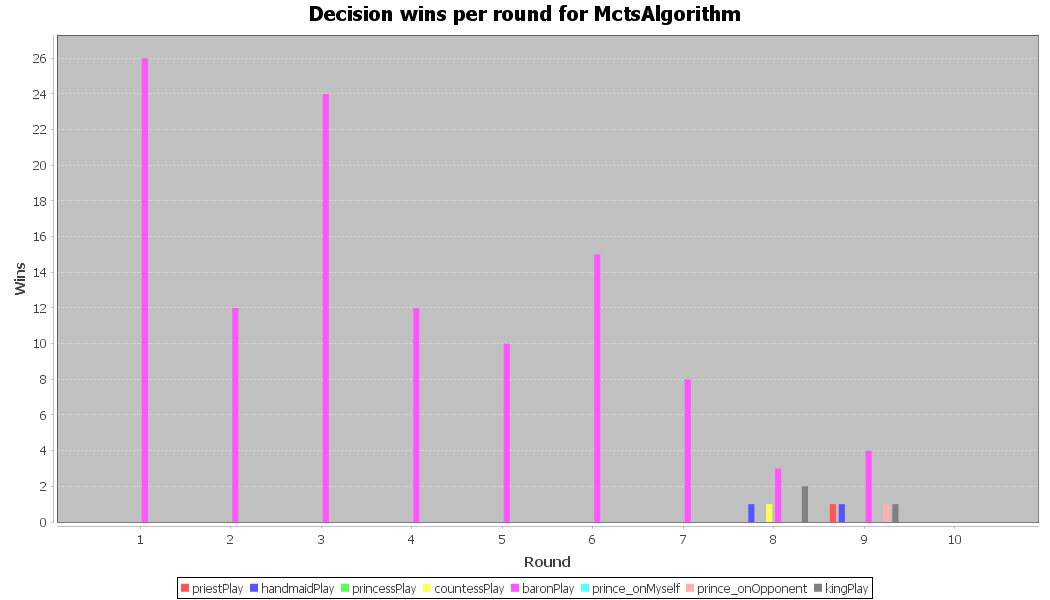
\includegraphics[width=\textwidth]{Resources/MirrorMctsVG/MctsVsGDecision.PNG}
	\caption{Wykres zwycięskich zagrań algorytmu MCTS} 
	\label{fig:MctsVsGDecision}
\end{figure} 

\begin{figure}[H]
	\centering
	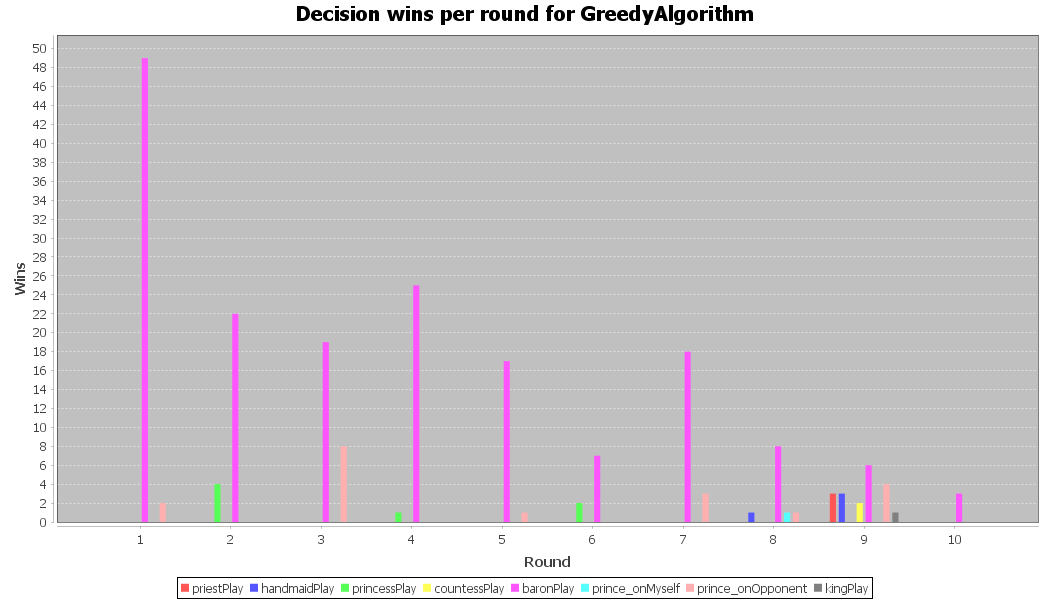
\includegraphics[width=\textwidth]{Resources/MirrorMctsVG/GVsMctsDecision.PNG}
	\caption{Wykres zwycięskich zagrań algorytmu zachłannego} 
	\label{fig:GVsMctsDecision}
\end{figure} 

Powyższe wykresy (rys. \ref{fig:MctsVsGDecision} i \ref{fig:GVsMctsDecision}) zwracają uwagę na nieregularność algorytmu MCTS do zwyciężania zagraniem karty Baron. Może to wynikać z tego, że MCTS częściej zatrzymuje w ręce kartę o wyższym numerze, i kiedy przeciwnik zagrywa kartę Barona, przegrywa.

\begin{figure}[H]
	\centering
	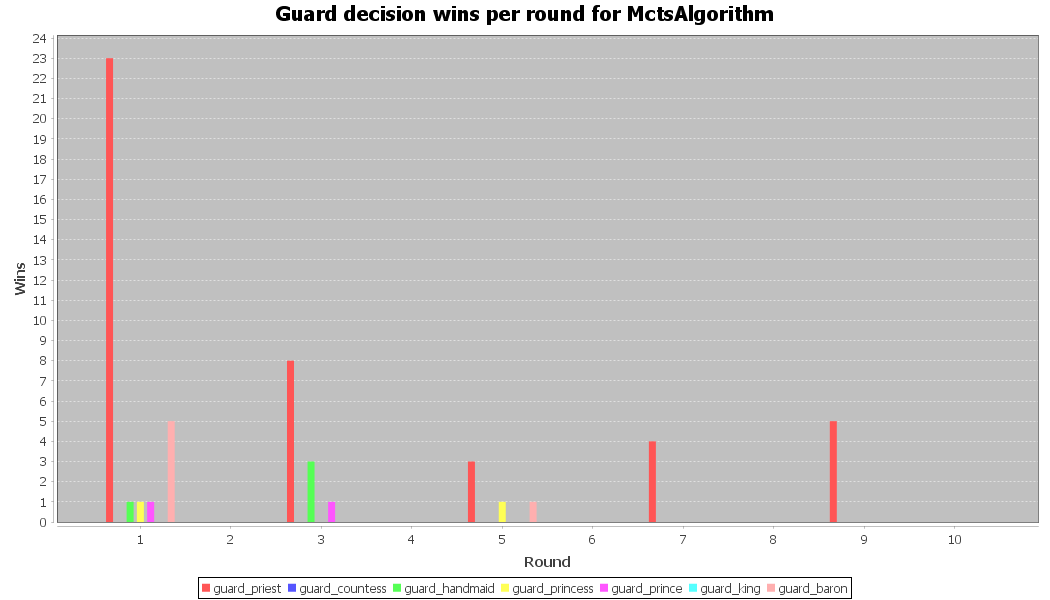
\includegraphics[width=\textwidth]{Resources/MirrorMctsVg/MctsVsGGuardDecision.PNG}
	\caption{Wykres szczegółowy zwycięskich zagrań karty Strażniczki} 
	\label{fig:MctsVsGGuardDecision}
\end{figure}

\begin{figure}[H]
	\centering
	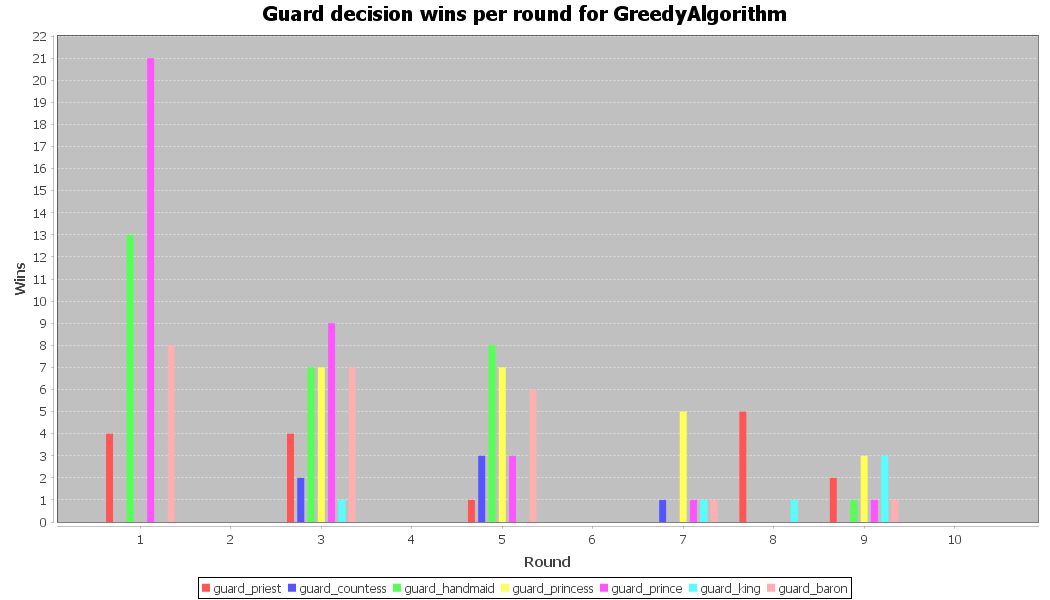
\includegraphics[width=\textwidth]{Resources/MirrorMctsVg/GVsMctsGuardDecision.PNG}
	\caption{Wykres szczegółowy zwycięskich zagrań karty Strażniczki} 
	\label{fig:GVsMctsGuardDecision}
\end{figure}

Na powyższych wykresach (rys. \ref{fig:MctsVsGGuardDecision} i \ref{fig:GVsMctsGuardDecision}) można zauważyć zupełnie inne tendencje do zagrywania karty Strażniczki. Algorytm MCTS niemal zawsze wybiera kartę Kapłana, natomiast algorytm zachłanny mimo że preferuje wybór Księcia, to niemal równie często wybiera inne typy kart.

\section{Algorytm Minimaksowy versus Algorytm MCTS}

\begin{figure}[H]
	\centering
	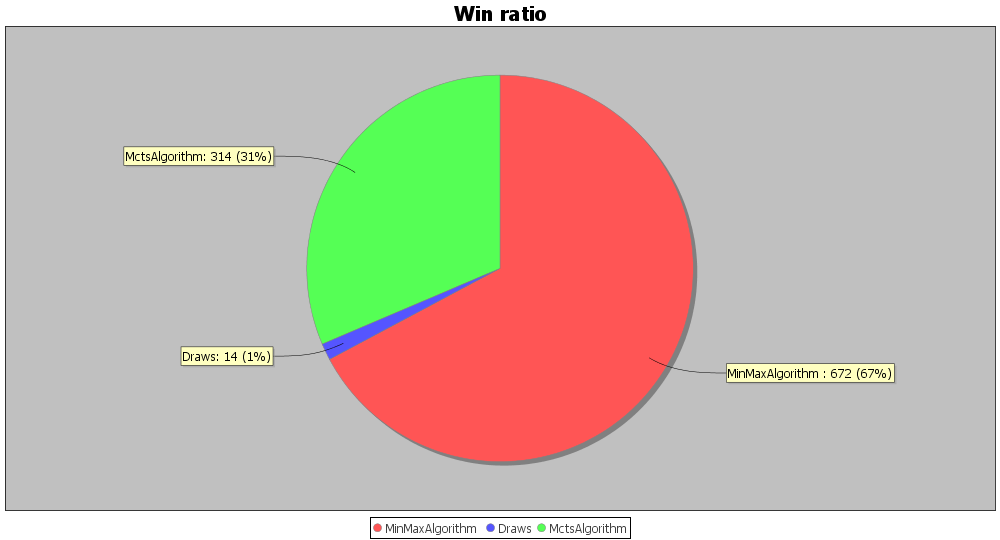
\includegraphics[width=\textwidth]{Resources/MirrorMmVsMcts/MmVsMctsWin.PNG}
	\caption{Wykres kołowy zwycięstw i remisów} 
	\label{fig:MmVsMctsWin}
\end{figure}

\begin{figure}[H]
	\centering
	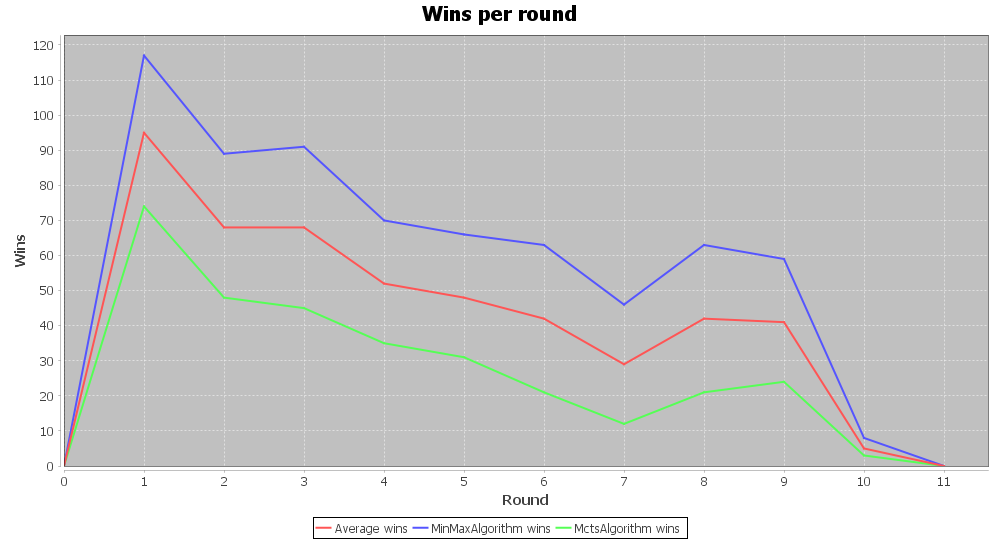
\includegraphics[width=\textwidth]{Resources/MirrorMmVsMcts/MmVsMctsRoundWin.PNG}
	\caption{Wykres wygranych w danej rundzie} 
	\label{fig:MmVsMctsRoundWin}
\end{figure}

Powyższe wykresy (rys. \ref{fig:MmVsMctsWin} i \ref{fig:MmVsMctsRoundWin}) pokazują przewagę algorytmu minimaksowego nad algorytmem MCTS.

\begin{figure}[H]
	\centering
	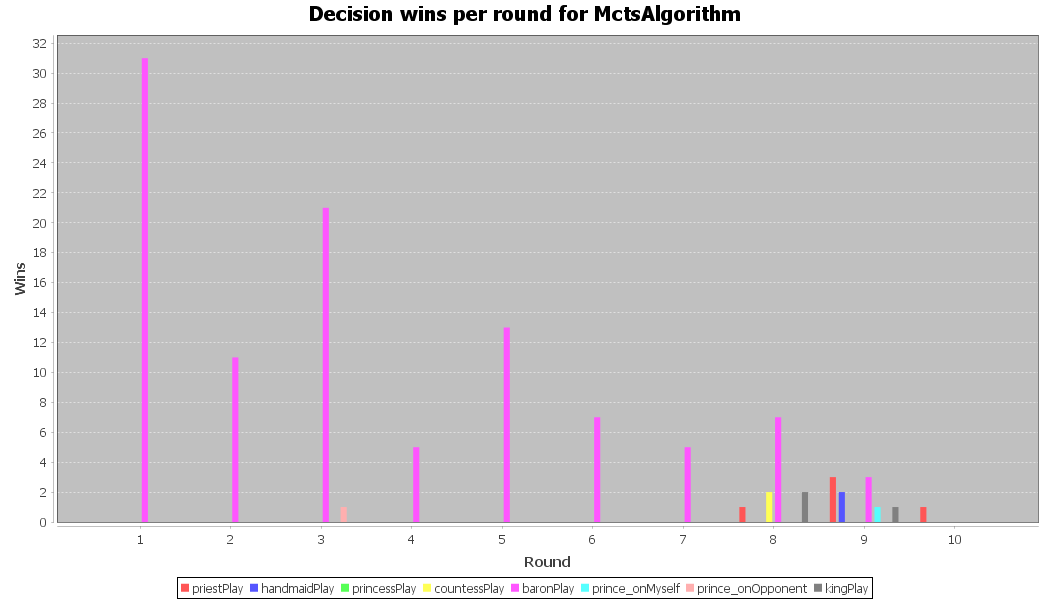
\includegraphics[width=\textwidth]{Resources/MirrorMmVsMcts/MctsVsMmDecision.PNG}
	\caption{Wykres zwycięskich zagrań algorytmu MCTS} 
	\label{fig:MctsVsMmDecision}
\end{figure} 

\begin{figure}[H]
	\centering
	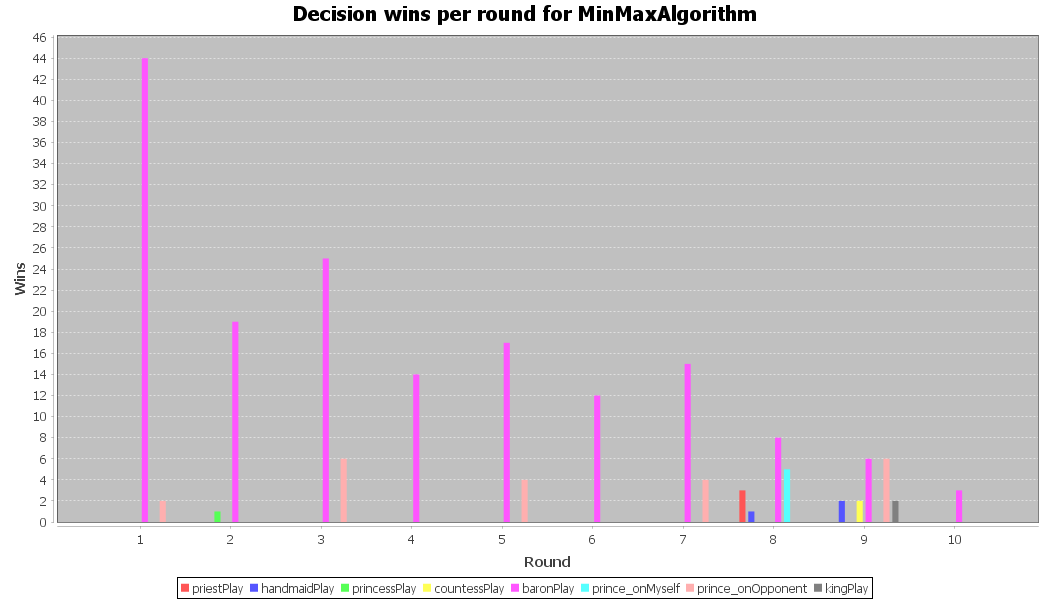
\includegraphics[width=\textwidth]{Resources/MirrorMmVsMcts/MmVsMctsDecision.PNG}
	\caption{Wykres zwycięskich zagrań algorytmu zachłannego} 
	\label{fig:MmVsMctsDecision}
\end{figure} 

Na powyższych wykresach (rys. \ref{fig:MctsVsMmDecision} i  \ref{fig:MmVsMctsDecision}) warto zwrócić uwagę na statystykę zwycięskich zagrań w ostatnich rundach. Algorytm minimaksowy do końca zagrywa karty Barona i często wykorzystuje Księcia. Zwycięskie zagrania algorytmu MCTS w ostatnich rundach są bardziej równomiernie rozłożone, a w ostatniej rundzie nigdy nie zagrywa karty Barona.

\begin{figure}[H]
	\centering
	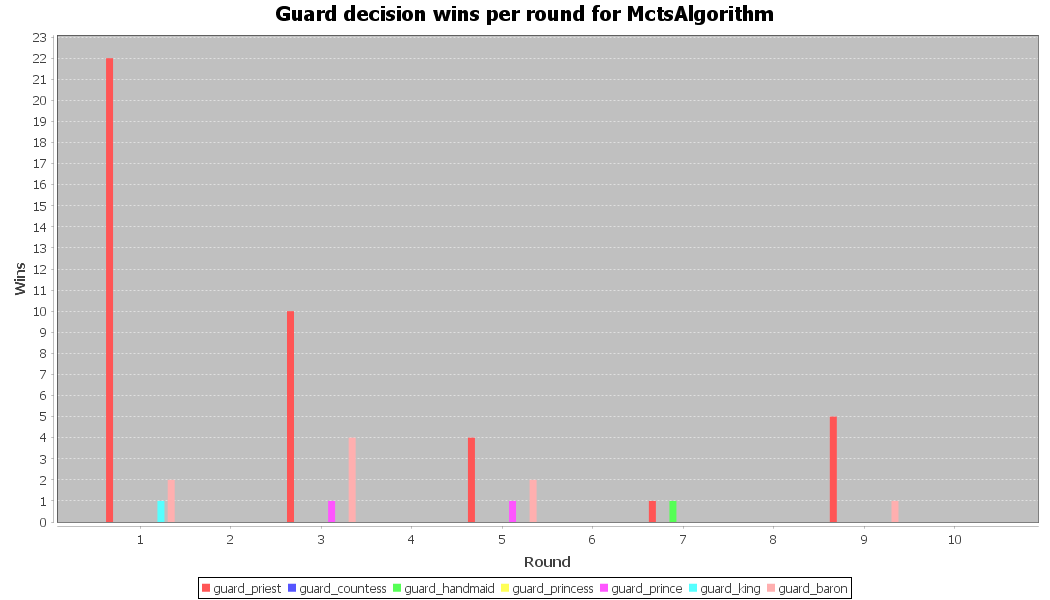
\includegraphics[width=\textwidth]{Resources/MirrorMmVsMcts/MctsVsMmGuardDecision.PNG}
	\caption{Wykres szczegółowy zwycięskich zagrań karty Strażniczki} 
	\label{fig:MctsVsMmGuardDecision}
\end{figure}

\begin{figure}[H]
	\centering
	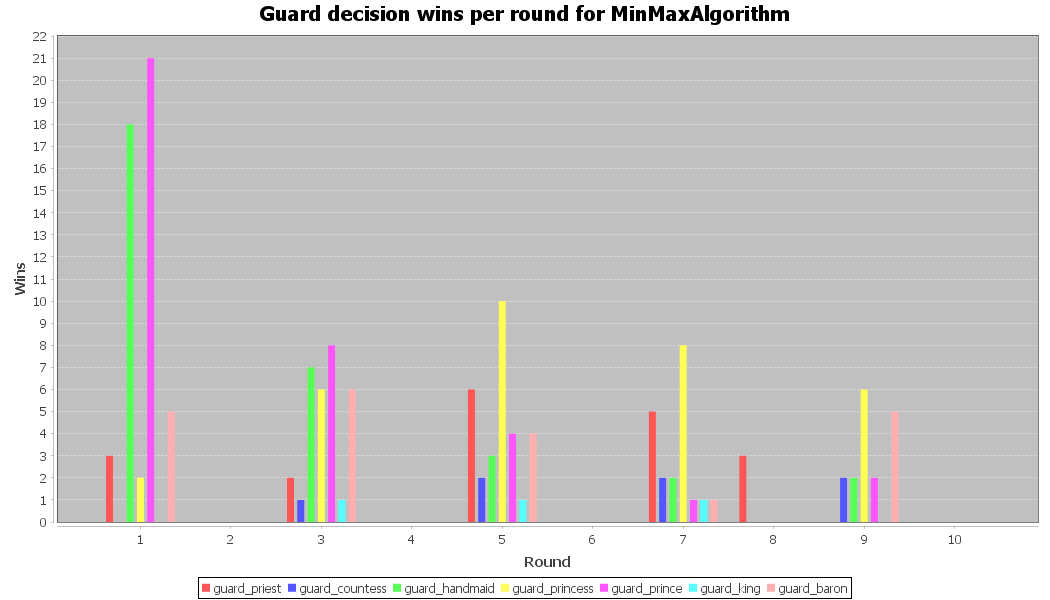
\includegraphics[width=\textwidth]{Resources/MirrorMmVsMcts/MmVsMctsGuardDecision.PNG}
	\caption{Wykres szczegółowy zwycięskich zagrań karty Strażniczki} 
	\label{fig:MmVsMctsGuardDecision}
\end{figure}

Na powyższych wykresach (rys. \ref{fig:MctsVsMmGuardDecision} i \ref{fig:MmVsMctsGuardDecision}) widać, że algorytm MCTS zachowuje się podobnie jak wcześniej, natomiast algorytm minimaksowy zdecydowanie częściej zagrywa kartę Strażniczki z wyborem Księżniczki niż w było to w przypadku algorytmu zachłannego.

\section{Wnioski}
Na podstawie przeprowadzonych badań można sformułować następujące wnioski:
\begin{enumerate}
	\item Zdecydowana większość gier kończy się w pierwszych 3 rundach, głównie poprzez zagranie kart Strażniczki i Barona. Wynika z tego również, że gracz rozpoczynający ma znaczną przewagę nad drugim graczem.
	\item W kolejnych rundach średnia ilość zwycięstw maleje, a następnie rośnie w dwóch ostatnich. Wynika to z dwóch zjawisk: po pierwsze, przy końcu gry gracze wyzbyli się już kart ofensywnych, czyli Strażniczki, Barona i Księcia, wobec czego dochodzi do porównania sił kart. Po drugie, jeśli karty ofensywne pozostały grze, znacznie wzrasta skuteczność ich użycia, co widać po częstości zagrań Strażniczki ze wskazaniem na Księżniczkę, bądź Księcia ze wskazaniem na przeciwnika (spodziewając się, że ma Księżniczkę).
	\item Ze statystyk można wywnioskować, że gra zdecydowanie sprzyja ofensywnym zagraniom.
	\item Algorytm losowy nie wymaga głębokiej analizy - niemniej jednak warty uwagi jest fakt, że jest bardziej skuteczny niż algorytm MCTS.
	\item Algorytm zachłanny osiąga wysokie wyniki w porównaniu z innymi algorytmami i niewiele niższe niż algorytm minimaksowy. Wynika to ze wspomnianego faworyzowania przez grę zagrań, które jak najszybciej zakończą grę. 
	\item Algorytm minimaksowy osiąga wyniki tylko niewiele lepsze niż algorym zachłanny, pomimo znacznie dłuższego czasu działania. Warto pamiętać, że w przedstawionym wariancie dokonuje on tylko przeszukania drzewa rozwiązań do 1 ruchu w przód. Algorytm ten osiąga przewagę nad zachłannym w rundach środkowych, jednak różnica zwycięstw jest niewielka.
	\item Efektywność algorytmu Monte Carlo Tree Search jest zdecydowanie poniżej oczekiwań, co widać szczególnie po wynikach eksperymentu z algorytmem losowym. Przyczyną tego stanu rzeczy jest moje błędne założenie, że negatywny wpływ elementu losowego na algorytm może zostać zniwelowany przez ilość symulacji przeprowadzanych przez MCTS. Niestety, implementacja algorytmu w formie podstawowej sprawia, że wpada on w pewną pułapkę już podczas pierwszego kroku. Jest to spowodowane tym, że gracz w danym momencie gry nie zna całego jej stanu, lecz zbiór informacyjny $I_k$, w związku z tym w korzeniu drzewa zawarty jest jeden wylosowany stan z tego zbioru informacyjnego. Biorąc pod uwagę ilość stanów w tym zbiorze, szansa, że zostanie wylosowany ten faktyczny, jest niewielka. Każda symulacja wykonana na błędnie założonym stanie początkowym w korzeniu drzewa algorytmu MCTS będzie prowadzić do błędnych wniosków. W efekcie MCTS osiąga gorsze wyniki niż algorytm losowy. Można by to podsumować potocznym stwierdzeniem, że ,,lepszy jest brak wiedzy, niż wiedza nieprawdziwa".
\end{enumerate}

\chapter{Podsumowanie}
\label{cha:rozdz6}

Celem mojej pracy była analiza i porównanie efektywności wybranych algorytmów w podejmowaniu decyzji w grze ,,Love Letter''. Podstawowym założeniem było nie przeszukiwanie całego drzewa rozwiązań, lecz jedynie najbliższy poziom, bądź posłużenie się heurystyką.

Opisałem zasady gry ,,Love Letter'', a następnie oszacowałem ilość możliwych rozwiązań. Na tej podstawie przedstawiłem ją jako problem optymalizacyjny, który stał się podstawą do porównania efektywności algorytmów. Model gry zapisałem w postaci gry ekstensywnej opierając się na Teorii Gier.

Do analizy i porównania wybrałem następujące algorytmy: losowy, zachłanny, minimaksowy oraz Monte Carlo Tree Search, który jest algorytmem heurystycznym. Sposób działania każdego z nich został opisany i podałem przykłady ich wykorzystania w praktyce. Następnie zaprezentowałem pomysł ich użycia do podejmowania decyzji w grze ,,Love Letter''.

Kolejno zaprezentowałem założenia programu, w którym zaimplementowane zostały zasady gry oraz wspomniane algorytmy. Przedstawiłem analizę wymagań oraz diagramy objaśniające strukturę programu. W analizie post implementacyjnej wskazałem główny problem związany z napisaniem programu, jakim okazał się niedostateczny poziom abstrakcji, znacznie zwiększający objętość kodu i tym samym ryzyko popełnienia błędu.

Następnie zaprezentowałem wyniki przeprowadzonych przeze mnie symulacji gier. W analizie skupiłem się na ilości zwycięstw danego algorytmu oraz najczęściej wygrywających zagraniach. Ważnym wnioskiem było wskazanie najskuteczniejszego z analizowanych algorytmów, jakim okazała się moja implementacja algorytmu minimaksowego. Z pewnością jego skuteczność mogłaby być wyższa, jednak z racji charakteru gry, który preferuje szybkie kończenie rund ponad zagrywki przedłużające grę, czas działania algorytmu rósł by zdecydowanie szybciej niż jego efektywność. 

Największym zaskoczeniem są wyniki algorytmu MCTS, gorsze nawet od wyników algorytmu losowego. Taki stan rzeczy wynika z błędnie przyjętych na początku założeń, że podstawowa wersja tego algorytmu będzie w stanie osiągać dobre wyniki w tej grze. Mimo to uważam, że po odpowiedniej modyfikacji polegającej na zamianie stanów znajdujących się w węzłach na zbiory informacyjne, byłby on w stanie osiągać wyniki równe, a nawet lepsze, od algorytmu minimaksowego.

\bibliographystyle{alpha}

\begin{thebibliography}{1}

\bibitem{}
\label{bib:loveLetterGame}
Alderac Entertainment Group,
\newblock {\em Love Letter},
\newblock 2012.

\bibitem{}
\label{bib:loveLetterWebsite}
Alderac Entertainment Group,
\newblock {\em Love Letter},
\newblock http://www.alderac.com/tempest/love-letter, 2016-02-08.

\bibitem{}
\label{bib:tabliceMatematyczne}
Alicja Cewe, Halina Nahorska, Irena Pancer,
\newblock {\em Tablice matematyczne},
\newblock Wydawnictwo Podkowa, Gdańsk 2002,
\newblock rozdział {\em Kombinatoryka}.

\bibitem{}
\label{bib:wiki_ProblemOptymalizacyjny}
\newblock {\em Wikipedia}, hasło {\em Problem optymalizacyjny}.
\newblock https://pl.wikipedia.org/wiki/Problem\_optymalizacyjny, 2016-02-21.

\bibitem{}
\label{bib:wiki_StrategiaTeoriaGier}
\newblock {\em Wikipedia}, hasło {\em Strategia w teorii gier}.
\newblock https://pl.wikipedia.org/wiki/Strategia\_mieszana, 2016-04-10.

\bibitem{}
\label{bib:matematyczneModeleKonfliktu_klasyfikacja}
Andrzej Z. Grzybowski
\newblock {\em Matematyczne modele konfliktu. Wykłady z Teorii Gier i Decyzji},
\newblock Wydawnictwo Politechniki Częstochowskiej, Częstochowa 2012,
\newblock rozdział {\em 1.1 Klasyfikacja problemów decyzyjnych}.

\bibitem{}
\label{bib:matematyczneModeleKonfliktu_graEkstensywna}
Andrzej Z. Grzybowski
\newblock {\em Matematyczne modele konfliktu. Wykłady z Teorii Gier i Decyzji},
\newblock Wydawnictwo Politechniki Częstochowskiej, Częstochowa 2012,
\newblock rozdział {\em 2.1 Gry w postaci ekstensywnej}.

\bibitem{}
\label{bib:wiki_drzewo}
\newblock {\em Wikipedia}, hasło {\em Drzewo (matematyka)}.
\newblock https://pl.wikipedia.org/wiki/Drzewo\_(matematyka), 2016-06-01.

\bibitem{}
\label{bib:wiki_TeoriaDecyzji}
\newblock {\em Wikipedia}, hasło {\em Teoria decyzji}.
\newblock https://pl.wikipedia.org/wiki/Teoria\_decyzji, 2016-04-10.

\bibitem{}
\label{bib:algorytmy_zachlanny}
Sanjoy Dasgupta, Christos Papadimitriou, Umesh Vazirani,
\newblock {\em Algorytmy},
\newblock Wydawnictwo Naukowe PWN, Warszawa 2012,
\newblock rozdział {\em Algorytmy Zachłanne}, s. 133.

\bibitem{}
\label{bib:wiki_minMax}
\newblock {\em Wikipedia}, hasło {\em Algorytm min-max}.
\newblock https://pl.wikipedia.org/wiki/Algorytm\_min-max, 2016-04-24.


\bibitem{}
\label{bib:minMax_warcaby}
\newblock {\em Funkcja oceniająca do algorytmu minimaksu w grze warcaby},
\newblock http://sequoia.ict.pwr.wroc.pl/~witold/aiarr/2009\_projekty/warcaby/, 2016-05-04.

\bibitem{}
\label{bib:wazniak_minMax}
\newblock {\em Studia Informatyczne}, Sztuczna inteligencja/SI Moduł 8 - Gry dwuosobowe.
\newblock http://wazniak.mimuw.edu.pl/index.php?title=Sztuczna\_inteligencja\/SI\_Moduł\_8\_-\_Gry\_dwuosobowe, 2016-04-24.

\bibitem{}
\label{bib:mcts_hex}
Broderick Arneson, Ryan Hayward, Philip Henderson,
\newblock {\em MoHex Wins Hex Tournament},
\newblock ICGA Journal Vol. 32 No. 2 s. 114–116, Czerwiec 2009

\bibitem{}
\label{bib:wiki_mcts}
\newblock {\em Wikipedia}, hasło {\em Monte-Carlo Tree Search}.
\newblock https://pl.wikipedia.org/wiki/Monte-Carlo\_Tree\_Search, 2016-05-04.

\bibitem{}
\label{bib:mcts_wprowadzenie}
\newblock {\em Introduction to Monte Carlo Tree Search},
\newblock https://jeffbradberry.com/posts/2015/09/intro-to-monte-carlo-tree-search/, 2016-05-04.

\bibitem{}
\label{bib:mcts_opis}
Guillaume Chaslot, Sander Bakkes, Istvan Szita, Pieter Spronck,
\newblock {\em Monte-Carlo Tree Search: A New Framework for Game AI},
\newblock Universiteit Maastricht / MICC.
\newblock P.O. Box 616, NL-6200 MD Maastricht, The Netherlands

\bibitem{}
\label{bib:mcts_totalWar}
\newblock {\em Monte-Carlo Tree Search in TOTAL WAR: ROME II’s Campaign AI},
\newblock http://aigamedev.com/open/coverage/mcts-rome-ii/, 2016-05-04.

\bibitem{}
\label{bib:mcts_osadnicy}
Istvan Szita, Guillaume Chaslot, Pieter Spronck,
\newblock {\em Monte-Carlo Tree Search in Settlers of Catan} 
\newblock Volume 6048 of the series Lecture Notes in Computer Science, s. 21-32, 2010.

\bibitem{}
\label{bib:mcts_uct}
\newblock {\em Monte Carlo Tree Search}, sekcja {\em About},
\newblock http://www.cameronius.com/research/mcts/about/index.html, 2016-05-05.

\bibitem{}
\label{bib:analiza_wymagan}
Krzysztof Sacha
\newblock {\em Inżynieria oprogramowania}
\newblock Wydawnictwo Naukowe PWN, Warszawa 2014,
\newblock rozdział {\em Inżynieria wymagań}, s. 50.

\bibitem{}
\label{bib:wiki_wierszPolecen}
\newblock {\em Wikipedia}, hasło {\em Wiersz poleceń}.
\newblock https://pl.wikipedia.org/wiki/Wiersz\_poleceń, 2016-05-08.

\bibitem{}
\label{bib:java}
Oracle Corporation
\newblock {\em Java}
\newblock http://www.oracle.com/technetwork/java/javase/downloads/index.html, 2016-05-08.

\bibitem{}
\label{bib:analiza_wymagan}
Krzysztof Sacha
\newblock {\em Inżynieria oprogramowania}
\newblock Wydawnictwo Naukowe PWN, Warszawa 2014,
\newblock rozdział {\em Metodyka zwinna}, s. 334.

\bibitem{}
\label{bib:wiki_waterfall}
\newblock {\em Wikipedia}, hasło {\em Model kaskadowy}.
\newblock https://pl.wikipedia.org/wiki/Model\_kaskadowy, 2016-05-08.
	
\bibitem{}
\label{bib:intellij}
JetBrains
\newblock {\em IntelliJ IDEA}
\newblock https://www.jetbrains.com/idea/, 2016-05-08.

\bibitem{}
\label{bib:czysty_kod}
Robert C. Martin
\newblock {\em Czysty Kod}
\newblock Wydawnictwo Helion, Gliwice 2014


\bibitem{}
\label{bib:czysty_kod_cytat_booch}
Robert C. Martin
\newblock {\em Czysty Kod}
\newblock Wydawnictwo Helion, Gliwice 2014,
\newblock rozdział 1. {\em Czysty Kod}, s. 30.

\bibitem{}
\label{bib:wiki_SOLID}
\newblock {\em Wikipedia}, hasło {\em SOLID (programowanie obiektowe)}.
\newblock https://pl.wikipedia.org/wiki/SOLID\_(programowanie\_obiektowe), 2016-06-28.

\end{thebibliography}
\end{document}
